\documentclass[12pt,a4paper]{article}

% ---------- Packages ----------
\usepackage[most]{tcolorbox}
\usepackage{graphicx}
\usepackage[T1]{fontenc}
\usepackage[utf8]{inputenc}
\usepackage[margin=1in]{geometry}
\usepackage{microtype}
\usepackage{lmodern}
\usepackage{mathtools,amsmath,amssymb,amsthm}
\usepackage{physics}
\usepackage{amsthm}
\usepackage{hyperref}
\usepackage[capitalize,noabbrev,nameinlink]{cleveref}
\usepackage{xcolor}
\usepackage{tikz}
\usepackage{booktabs}
\usepackage{siunitx}

\usetikzlibrary{arrows.meta,positioning,calc,decorations.pathreplacing}
\hypersetup{colorlinks=true,linkcolor=blue,citecolor=blue,urlcolor=blue}

% ---------- Theorems ----------
\newtheorem{axiom}{Axiom}
\newtheorem{definition}{Definition}
\newtheorem{proposition}{Proposition}
\newtheorem{theorem}{Theorem}
\newtheorem{conjecture}{Conjecture}
\newtheorem{remark}{Remark}
\newtheorem{example}{Example}
\newtheorem{corollary}{Corollary}
\newtheorem{lemma}{Lemma}
\newtheorem{assumption}{Assumption}

\crefname{axiom}{Axiom}{Axioms}
\crefname{definition}{Definition}{Definitions}
\crefname{theorem}{Theorem}{Theorems}
\crefname{proposition}{Proposition}{Propositions}
\crefname{lemma}{Lemma}{Lemmas}
\crefname{corollary}{Corollary}{Corollaries}

% Light notation hygiene
\newcommand{\Mset}{M}        % minimal set
% \newcommand{\order}{\prec}   % causal order
% \newcommand{\rank}{\mathrm{rk}}
\newcommand{\Kcs}{\Box_{\mathrm{cs}}}
\newcommand{\R}{\mathbb{R}}
\newcommand{\C}{\mathbb{C}}
\newcommand{\N}{\mathbb{N}}
\newcommand{\E}{\mathbb{E}}
\newcommand{\rk}{\mathrm{rk}}
\DeclareMathOperator{\Spin}{Spin}
\DeclareMathOperator{\Vol}{Vol}
% \tr is provided by physics; avoid redefining
% \DeclareMathOperator{\tr}{tr}

% ---------- Title ----------
\title{Emergent Reality from Size-Biased Order}
\author{VR}
\date{\today}


% === Convenience macro for 95% CIs ===
\newcommand{\ci}[2]{#1\,\pm\,#2}

\begin{document}
\maketitle

\begin{abstract}
  We develop a framework in which macroscopic reality emerges from a Hilbert space of potentials via a
  \emph{poset‐restricted, size‐biased sequential growth} with no background time. Latent arrival times are
  \emph{pure gauge}; the physical content is the induced total order and causal structure. From order and
  counts we recover Alexandrov topology and, in the continuum limit, Lorentzian geometry. We derive causal
  precedence from update‑locality, give concrete state‐process instantiations, obtain a Lindblad limit from
  weak Lüders‐type updates, and sketch a stress–energy estimator from link momenta. We include constants,
  finite‑$N$ effects, sandwich bounds for pairwise precedence, mass/coherence corrections, pseudocode and
  scripts for 1+1 and 3+1 sprinklings (with boost tests), and numerical tables validating the scaling laws.
\end{abstract}
  

\tableofcontents

\section{Foundational Axioms (Hilbert + Order-Only Randomness)}

\begin{axiom}[Potential Space and Intensity]\label{ax:potential}
Let $H$ be a separable complex Hilbert space with Borel $\sigma$-algebra $\mathcal{B}(H)$.
Fix a $\sigma$-finite Borel measure $\Lambda$ on $H$ and a measurable weight $w:H\to[0,\infty)$ with
$0<\int_H w(\psi)\, \Lambda(d\psi)<\infty$.
Define the intensity $\mu(d\psi):=w(\psi)\,\Lambda(d\psi)$.
\end{axiom}

\begin{axiom}[History-dependent marked point process; order is physical]\label{ax:prm}
There exists a marked point process $N$ on $H\times(0,\infty)$ whose \emph{predictable compensator} at rank/time $k$ has density $W(\psi;S_{k})\,\Lambda(d\psi)\,dt$. The induced total order $\triangleleft$ is by increasing latent time $t$, which is unphysical and gaugeable by any strictly increasing reparametrization. Only the induced order on events and the state-dependent selection from the current minimal set are physical.
\end{axiom}

\begin{proposition}[Countability and distinctness]
Almost surely, $\Pi$ has countably many atoms, hence $E$ is countable. If $\mu$ is atomless,
realized $\psi$'s are almost surely all distinct.
\end{proposition}

\begin{proposition}[Pairwise precedence (restricted race)]\label{prop:bt}
Let $A,B\in\mathcal B(H)$ be disjoint with $\mu(A),\mu(B)>0$. In the \emph{restricted race} on $A\cup B$, the first arrival times $T_A,T_B$ satisfy
\[\mathbb P(T_A<T_B)=\frac{\mu(A)}{\mu(A)+\mu(B)}.\]
For a finite labeled set $\{\psi_i\}$ with $\mu(\{\psi_i\})=w(\psi_i)>0$, the arrival times $T_i$ are independent exponentials with rates $w(\psi_i)$ and $\mathbb P(T_i<T_j)=\frac{w(\psi_i)}{w(\psi_i)+w(\psi_j)}$.
\end{proposition}

\begin{assumption}[Local summability \& unit-rate gauge]\label{ax:conservation-state}
There exists a measurable state space $(\mathsf S,\mathcal S)$, update map $\Phi:\mathsf S\times E\to\mathsf S$, and kernel $W:H\times\mathsf S\to[0,\infty)$ with $S_{k+1}=\Phi(S_k,e_{k+1})$ and $w^{(k)}(\psi)=W(\psi;S_k)$, such that for each $S$ and each antichain $A\subset H$, $\sum_{\psi\in A}W(\psi;S)<\infty$. We work in the \emph{unit-rate} time gauge, i.e.\ we reparametrize latent time so that $\int_H W(\psi;S_k)\,\Lambda(d\psi)\equiv 1$ for all $k$.
\end{assumption}

% \begin{lemma}[Random time change and gauge]\label{lem:time_change}
% Let $\lambda_k:=\int_H W(\psi;S_k)\,d\Lambda(\psi)$ be the predictable total rate before step $k$. The latent time parameter can be redefined by the (random) compensator $A_n=\sum_{k\le n}\lambda_k$, producing a unit-rate selection process. Since arrival times are unphysical (only $\triangleleft$ is), imposing $\int W(\psi;S_k)d\Lambda=\mathrm{const}$ is a gauge fixing, not an additional physical assumption.
% \end{lemma}
% \paragraph{Gauge fixing (unit rate).}
% By Lemma 1, the latent time parameter can always be
% % redefined so that the total rate \int_H W(\psi;S_k)\,d\Lambda(\psi) is constant. We henceforth adopt the
% % unit-rate gauge \int_H W(\psi;S_k)\,d\Lambda(\psi)\equiv 1 for all k.
% \begin{remark}[Clock gauge vs.\ rate conservation]\label{rem:gauge-vs-rate}
% Choosing the unit-rate clock is a \emph{reparametrization of latent time only}.
% In general, the total hazard \(\int_H W(\psi;S)\,d\Lambda(\psi)=\langle \mu(S),\Sigma\,\mu(S)\rangle\),
% with fixed covariance \(\Sigma:=\int \Phi\otimes\Phi\,d\Lambda\), depends on the current
% state \(\mu(S)\). Unless \(\Sigma=I\), the total rate is not dynamically conserved by the
% update; what is invariant is the induced \emph{order}. Claims of "conservation" below
% refer to the chosen clock gauge, not a dynamical invariant.
% \end{remark}

\begin{lemma}[Random time change and gauge]\label{lem:time-change}
Let \(\lambda_k:=\int_H W(\psi;S_k)\,d\Lambda(\psi)\) be the predictable total rate before step \(k\).
Redefining latent time by the compensator \(A_n=\sum_{j\le n}\lambda_j\) yields a unit‑rate selection
process. Since arrival times are unphysical (only the order is), imposing \(\int W\,d\Lambda=\text{const}\)
is a clock gauge, not a new physical assumption.
\end{lemma}

\paragraph{Gauge fixing (unit rate).}
By \cref{lem:time-change}, we can always reparametrize latent time so that
\(\int_H W(\psi;S_k)\,d\Lambda(\psi)\equiv 1\) for all \(k\).
\emph{Remark (clock gauge vs.\ rate conservation).} Choosing a unit‑rate clock is a reparametrization.
In general the total hazard \(\int_H W(\psi;S)\,d\Lambda(\psi)=\langle \mu(S),\,\Sigma\,\mu(S)\rangle\), with
\(\Sigma:=\int \Phi\otimes \Phi\,d\Lambda\), depends on state; it is \emph{not} dynamically conserved unless
\(\Sigma=I\). What is invariant is the induced order; any “conservation” below refers to the chosen clock gauge.


\begin{axiom}[Consistency]\label{ax:consistency}
Histories have nonzero probability only if they satisfy locality and gauge compatibility (formalized in \cref{sec:consistency}).
\end{axiom}

\input{consistency_early_v1}

\begin{axiom}[Accumulation]\label{ax:accumulation}
Actualizations, once realized, persist; the realized prefix $(E,\triangleleft)$ only grows.
\end{axiom}

\providecommand{\clref}[1]{\hyperref[cl:#1]{\textnormal{(CL#1)}}}

\begin{assumption}[Continuum-limit conditions]\label{ass:CL}
\leavevmode
\begin{enumerate}
  \item[(CL1)]\label{cl:1}\textbf{Retarded locality.}
  For every finite history $e$, there exists a measurable ``retarded region'' $\mathcal R(e)\subseteq H$
  (determined by $e$'s realized partial order, e.g., the down-set of the current minimal set)
  such that the update weight $k(e,\psi)$ vanishes off $\mathcal R(e)$.
  Moreover, $\mathcal R(e)$ is generated by a finite union of base elements from the Alexandrov basis,
  and its ``rank depth'' is uniformly bounded by a constant $D_{\mathrm{loc}}<\infty$.

  \item[(CL2)]\label{cl:2}\textbf{Finite-depth growth (non-explosion in rank).}
  There exists $C_{\mathrm{grow}}<\infty$ such that for every $e$,
  the expected number of admissible next events within $\mathcal R(e)$ is bounded by $C_{\mathrm{grow}}$,
  and along any chain the probability of seeing infinitely many new events in finite rank is zero.
  Equivalently, the layer counts in $\mathcal R(e)$ have uniformly bounded exponential moments.

  \item[(CL3)]\label{cl:3}\textbf{Approximate stationarity and isotropy at small scales.}
  For every $\varepsilon>0$ there exists a base scale $\delta>0$ such that for any Alexandrov
  element $A$ with ``diameter'' $\le \delta$ one has, uniformly over histories $e$ whose minimal
  set meets $A$,
  \[
    (1-\varepsilon)\,\mu(A) \;\le\; \mu_e(A) \;\le\; (1+\varepsilon)\,\mu(A),
  \]
  and directional averages of $\mu_e$ within $A$ deviate from those of $\mu$ by at most $\varepsilon$.
  (In words: locally, the history-updated mass is a small perturbation of the reference mass.)

  \item[(CL4)]\label{cl:4}\textbf{Density and scaling window.}
  There is a scaling parameter $n\to\infty$ and rescalings of base elements $A\mapsto A^{(n)}$
  such that the normalized measures $n^{-1}\mu_e(A^{(n)})$ converge in probability to a finite,
  nondegenerate limit density $\rho(A)$ uniformly on compact unions of base elements.
  Moreover, $0<\rho_{\min}\le \rho(A)\le \rho_{\max}<\infty$ locally.

  \item[(CL5)]\label{cl:5}\textbf{Stability (regularity of updates).}
  If two histories $e$ and $e'$ agree on the past within $\mathcal R(e)\cap\mathcal R(e')$
  up to rank depth $D_{\mathrm{stab}}$, then the total variation distance between their next-step
  kernels $K(e;\cdot)$ and $K(e';\cdot)$ is $o(1)$ at the scaling of \clref{4}.
  Equivalently, $k(e,\cdot)$ depends on $e$ in a locally Lipschitz way after coarse graining.
\end{enumerate}
\end{assumption}

\begin{remark}[Scope]\label{rem:CL_scope}
Conditions \clref{1}--\clref{5} are not needed for the \emph{existence/uniqueness} of the rank-time
process (Theorem~\ref{thm:eu}); they are invoked for continuum claims: retarded influence,
sandwich bounds, metric recovery, and curvature-from-layers.
\end{remark}


% ===================== Existence & Uniqueness (drop-in) =====================
\subsection{Existence and uniqueness of the history-dependent process}\label{subsec:eu}

We now justify Axiom~\ref{ax:prm} by exhibiting very mild conditions under which
a \emph{rank-time} realization exists and is unique in law. Time labels are a gauge:
once an ordered sequence $(\psi_n)_{n\ge 1}$ is constructed, any strictly increasing
clock can be attached to obtain a marked point process on $H\times(0,\infty)$.

\begin{assumption}[Admissible kernels and finiteness]\label{ass:EU}
Let $(H,\mathcal B(H))$ and the base intensity $\mu$ be as in Axiom~\ref{ax:potential}.
For each finite history $e=(\psi_1,\dots,\psi_m)\in H^m$, there is a Borel \emph{admissible set}
$S(e)\in\mathcal B(H)$ and a jointly measurable weight $k:H^{<\infty}\times H\to[0,\infty)$ such that
\begin{enumerate}
    \item[(EU1)] (\textbf{Support}) $k(e,\psi)=0$ for $\psi\notin S(e)$.
    \item[(EU2)] (\textbf{Finite, nonzero mass}) $0<\mu_e(H):=\int_{H} k(e,\psi)\,\mu(d\psi)<\infty$.
    \item[(EU3)] (\textbf{Measurability}) the set $\{(e,\psi):\psi\in S(e)\}$ is Borel in $H^{<\infty}\times H$ and
    $(e,\psi)\mapsto k(e,\psi)$ is jointly Borel measurable.\footnote{Here $H^{<\infty}:=\bigsqcup_{m\ge 0} H^m$
    is given the usual disjoint-union Borel $\sigma$-algebra.}
\end{enumerate}
Define the finite \emph{history-dependent measure} $\mu_e(A):=\int_A k(e,\psi)\,\mu(d\psi)$ on $\mathcal B(H)$.
\end{assumption}

\begin{definition}[One-step size-biased kernel]\label{def:kernel}
For a finite history $e$, write $M(e):=\mu_e(H)$ and define the stochastic kernel
\begin{equation}
    K(e;A)\;:=\;\frac{\mu_e(A)}{M(e)},\qquad A\in\mathcal B(H).
\end{equation}
This is the law of the next mark: the selection is \emph{size-biased} by the history-updated mass~$\mu_e$.
\end{definition}

\begin{theorem}[Rank-time existence and uniqueness]\label{thm:eu}
Under Assumption~\ref{ass:EU}, there exists a unique probability measure $\mathbb P$ on $(H^{\mathbb N},
\mathcal B(H)^{\otimes\mathbb N})$ and a process $(\psi_n)_{n\ge 1}$ such that for each $n\ge 1$ and $A\in\mathcal B(H)$,
\begin{equation}\label{eq:one_step}
    \mathbb P\!\left(\psi_n\in A \,\middle|\, \psi_{<n}=e\right)\;=\;K(e;A)\quad\text{almost surely.}
\end{equation}
Equivalently, $K$ is a family of one-step regular conditional probabilities for $(\psi_n)_{n\ge 1}$.
The law is unique in the sense of finite-dimensional distributions.
Moreover, there exists a Borel map $S:H^{<\infty}\times(0,1)\to H$ and i.i.d.\ $U_1,U_2,\dots\sim\mathrm{Unif}(0,1)$ such that
\begin{equation}
    \psi_n\,=\,S(\psi_{<n},U_n)\quad\text{for all }n\ge 1\quad\text{almost surely.}
\end{equation}
\end{theorem}

\begin{proof}[Proof sketch]
Because $K(\cdot;\cdot)$ is a Borel stochastic kernel on the Polish space $H$ (Assumption~\ref{ass:EU}),
the Ionescu--Tulcea extension theorem yields a unique measure on $H^{\mathbb N}$ under which
the cylinder probabilities are consistent and satisfy~\eqref{eq:one_step}.
The strong (functional) representation follows by standard measurable selection:
for each $e$, realize $K(e;\cdot)$ as the pushforward of a uniform random variable via some Borel selector $S(e,\cdot)$.
\end{proof}

\begin{corollary}[Embedding as a marked point process]\label{cor:embedding}
Fix any strictly increasing sequence $0<t_1<t_2<\cdots$ (a \emph{gauge clock}) and set
$N:=\sum_{n\ge 1}\delta_{(\psi_n,t_n)}$.
Then $N$ is a marked point process on $H\times(0,\infty)$ that satisfies Axiom~\ref{ax:prm},
and its physical order coincides with the rank order almost surely.
Alternatively, let $W_1,W_2,\dots$ be strictly positive (possibly history-dependent) waiting times with
$t_n=\sum_{j=1}^n W_j$. If $\sum_{n\ge 1} W_n=\infty$ almost surely (e.g.\ $W_n\equiv 1$), the embedding is non-explosive.
\end{corollary}

\begin{proposition}[Equivalence with restricted races]\label{prop:race_equiv}
Fix a finite history $e$ and a finite measurable partition $\{A_1,\dots,A_m\}$ of $S(e)$ with $\mu_e(A_i)<\infty$.
Consider the \emph{restricted race} in which we draw independent exponentials $T_i\sim\mathrm{Exp}(\lambda_i)$ with
$\lambda_i:=\mu_e(A_i)$ and declare the next mark to lie in the unique $A_i$ attaining $\min_j T_j$.
Then
\begin{equation}
    \mathbb P\!\left(\text{$A_i$ wins the race}\mid \psi_{<n}=e\right)\;=\;\frac{\lambda_i}{\sum_{j=1}^m \lambda_j}
    \;=\;K(e;A_i),
\end{equation}
so the race construction reproduces the one-step law~\eqref{eq:one_step}.
\end{proposition}

\begin{remark}[Minimality and locality]
Assumption~\ref{ass:EU}(EU2) is the only nontrivial finiteness requirement and is automatically satisfied if
$S(e)$ is relatively compact and $k(e,\cdot)$ is bounded there. If the dynamics are \emph{update-local}
(so $k(e,\cdot)$ depends on $e$ only through the current minimal set in the partial order),
the construction above remains valid verbatim. Conditions (CL1)--(CL5) are \emph{not} needed for existence/uniqueness;
they become relevant later for continuum limits.
\end{remark}
% ============================================================================


% \begin{tcolorbox}[title=Core model (one page), colback=white]
% \textbf{State:} kernel-mean \(\mu\in\mathcal{H}_K\) (Def.~\ref{def:kernel-mean-state}).\quad
% \textbf{Hazard:} \(W(\psi;S)=|\langle \psi,\mu\rangle|^2\).\\
% \textbf{Step:} choose \(e_{k+1}\in M(k)\) with \(\mathbb{P}(e_{k+1}=x\mid\mathcal{F}_k)\propto W(x;S_k)\);
% update \(\displaystyle \mu\mapsto \mu^+=\frac{(1-\eta)\mu+\eta\,\phi(e_{k+1})}{\|(1-\eta)\mu+\eta\,\phi(e_{k+1})\|}\)
% (Def.~\ref{def:local-rkhs-update}).\\
% \textbf{Gauge:} latent time reparametrized to unit total rate (Remark~\ref{rem:gauge-vs-rate}).\\
% \textbf{Locality:} \(K\) has bounded/decaying \(D\)-range; influence obeys Prop.~\ref{prop:leakage}.\\
% \textbf{Continuum:} (CL1)–(CL5) \(\Rightarrow\) metric recovery (Thm.~4).
% \end{tcolorbox}

\begin{quote}\small
\textbf{Core model (one page).}\;
\emph{State:} kernel‑mean \(m\in\mathcal H_K\).
\;\; \emph{Hazard:} \(W(\psi;S)=|\langle \psi, m\rangle|^2\).
\;\; \emph{Step:} choose \(e_{k+1}\in \Mset(k)\) with \(\Pr(e_{k+1}=x\mid\mathcal F_k)\propto W(x;S_k)\);
update \(m\mapsto m^+=(1-\eta)m+\eta\,\phi(e_{k+1})\), normalized.
\;\; \emph{Gauge:} reparametrize latent time to unit total rate.
\;\; \emph{Locality:} kernel has bounded/decaying \(D\)-range; influence obeys exponential leakage bounds.
\;\; \emph{Continuum:} (CL1)–(CL5) \(\Rightarrow\) metric recovery.
\end{quote}
  
% ===================== Symbols & units (drop-in table) =====================
% Requires: \usepackage{booktabs} (already in preamble). Optionally: siunitx.
\begin{table}[t]
\centering
\caption{Symbols, meanings, and (where applicable) physical units.}
\label{tab:symbols}
\begin{tabular}{@{}lllc@{}}
\toprule
\textbf{Symbol} & \textbf{Meaning} & \textbf{Notes} & \textbf{Units} \\
\midrule
$H$ & Potential space of marks & Standard Borel / Polish & -- \\
$\mathcal B(H)$ & Borel $\sigma$-algebra on $H$ & -- & -- \\
$\mu$ & Base intensity (reference measure) & $\sigma$-finite; finite on compacta (assumed) & depends on $H$ \\
$e=(\psi_1,\dots,\psi_m)$ & Finite history (rank prefix) & Order is physical & -- \\
$k(e,\psi)$ & History-dependent weight & jointly measurable; update-local & -- \\
$\mu_e(A)=\int_A k(e,\psi)\,d\mu$ & Updated measure & finite and nonzero by (EU2) & -- \\
$M(e)=\mu_e(H)$ & Total updated mass & normalizer & -- \\
$K(e;A)=\mu_e(A)/M(e)$ & One-step kernel (next mark) & size-biased selection & -- \\
$N=\sum_n\delta_{(\psi_n,t_n)}$ & Marked point process & gauge clock $(t_n)$ strictly increasing & -- \\
$K(\psi,\psi')$ & PSD kernel on $H$ & RKHS kernel & -- \\
$\Phi(\psi)$ & RKHS feature map & $K(\psi,\psi')=\langle\Phi(\psi),\Phi(\psi')\rangle$ & -- \\
$m_e=\int \Phi\,dP_e$ & Kernel-mean state & $\|m_e\|\le\sqrt{\kappa}$ & -- \\
$\beta$ & Update strength & enters $u=\exp\{\beta r\}$ & dimensionless \\
$\ell$ & Kernel length scale & e.g., Gaussian kernel & same as $H$'s length \\
$\rho$ & Limit density (CL4) & $n^{-1}\mu_e(A^{(n)})\to \rho(A)$ & depends on scaling \\
$D_{\mathrm{loc}}$ & Locality rank-depth bound (CL1) & retarded region depth & rank \\
$C_{\mathrm{grow}}$ & Growth bound (CL2) & exp.\ moment control & -- \\
$Z_e(\psi_n)$ & Update normalizer & $=\int u(\psi;\psi_n)\,dP_e$ & -- \\
$u(\psi;\psi_n)$ & Multiplicative update factor & $>0$; $=\exp\{\beta r\}$ in examples & -- \\
$\Lambda$ & Base measure on $H$ & fixed reference; $\mathrm{units}(\Lambda)\!\times\!\mathrm{units}(W)$ matches rate & -- \\
$W(\psi;S)$ & event hazard & state-dependent; integrates to a rate density & rate density \\

\bottomrule
\end{tabular}
\end{table}

\subsection{RKHS setup and kernel-mean state}\label{subsec:rkhs}

Let $(H,\mathcal B(H))$ be as above and let $K:H\times H\to\mathbb R$ be a bounded,
measurable, positive-semidefinite (PSD) kernel with $\sup_{x} K(x,x)\le \kappa<\infty$.
Let $\mathcal H_K$ denote the reproducing-kernel Hilbert space (RKHS) with feature map
$\Phi:H\to\mathcal H_K$, $\Phi(\psi):=K(\,\cdot\,,\psi)$, so that
$K(\psi,\psi')=\langle \Phi(\psi),\Phi(\psi')\rangle_{\mathcal H_K}$.

For a finite history $e$, recall the finite \emph{history-dependent measure}
$\mu_e(A)=\int_A k(e,\psi)\,\mu(d\psi)$ (Assumption~\ref{ass:EU}) and its normalized law
$P_e:=\mu_e/M(e)$ with $M(e)=\mu_e(H)$.

\begin{definition}[Kernel mean state]\label{def:kernel-mean-state}
The \emph{kernel mean} (state) associated with $e$ is
\begin{equation}
  m_e \;:=\; \int_H \Phi(\psi)\,P_e(d\psi) \;\in\; \mathcal H_K.
\end{equation}
For any $f\in\mathcal H_K$, expectations are represented by
$\mathbb E_{P_e}[f(\Psi)] \;=\; \langle f,\, m_e\rangle_{\mathcal H_K}$.
\end{definition}

\begin{proposition}[Existence and boundedness]\label{prop:kme_exists}
If $K$ is bounded and measurable, then $m_e$ exists for every finite history $e$ and
$\|m_e\|_{\mathcal H_K}\le \sqrt{\kappa}$. In particular, $m_e$ is well-defined regardless of the cardinality of~$H$.
\end{proposition}

\begin{proof}[Sketch]
Since $\|\Phi(\psi)\|^2=K(\psi,\psi)\le \kappa$ and $\Phi$ is measurable, the Bochner integral
$\int \Phi(\psi)\,P_e(d\psi)$ exists and has norm at most $\sqrt{\kappa}$.
\end{proof}

\paragraph{Bridge to GNS.}
Let $\omega_e:C_b(H)\to\mathbb R$ be the positive linear functional $\omega_e(f)=\int f(\psi)\,P_e(d\psi)$.
By the GNS construction there exists a cyclic representation $(\pi_e,\mathcal H_e,\xi_e)$ with
$\omega_e(f)=\langle \xi_e,\,\pi_e(f)\xi_e\rangle$. When $f(\cdot)=\langle g,\Phi(\cdot)\rangle_{\mathcal H_K}$
for some $g\in\mathcal H_K$, the RKHS representation recovers the same expectation via $m_e$.
This provides a concrete bridge from the order-updated law $P_e$ to Hilbert structure.

\subsubsection*{Exact and first-order update of $m_e$}
Let $e^+=e\cup\{\psi_n\}$. Suppose the update is \emph{multiplicative}:
there exists a strictly positive, measurable factor $u(\cdot;\psi_n)$ such that
\begin{equation}\label{eq:mult_update}
  k(e^+,\psi) \;=\; k(e,\psi)\,u(\psi;\psi_n),\qquad \psi\in H.
\end{equation}
Then with $Z_e(\psi_n):=\int u(\psi;\psi_n)\,P_e(d\psi)$ the normalized next law is
$P_{e^+}(d\psi)=\frac{u(\psi;\psi_n)}{Z_e(\psi_n)}\,P_e(d\psi)$ and
\begin{equation}\label{eq:exact_update}
  m_{e^+} \;=\; \frac{\displaystyle \int \Phi(\psi)\,u(\psi;\psi_n)\,P_e(d\psi)}
                      {\displaystyle \int u(\psi;\psi_n)\,P_e(d\psi)}.
\end{equation}

\begin{proposition}[First-order (small-$\beta$) formula]\label{prop:first_order}
If $u(\psi;\psi_n)=\exp\!\{\beta\,r(\psi;\psi_n)\}$ with $r$ bounded and $\beta$ small, then
\begin{equation}\label{eq:first_order}
  m_{e^+} \;=\; m_e \;+\; \beta\,\mathrm{Cov}_{P_e}\!\big[\Phi(\Psi),\, r(\Psi;\psi_n)\big] \;+\; O(\beta^2).
\end{equation}
In particular, for $r(\psi;\psi_n)=K(\psi,\psi_n)$ the update moves $m_e$ in the direction of
the centered feature $\Phi(\psi)$ correlated with the kernel bump at $\psi_n$.
\end{proposition}

\begin{proof}[Sketch]
Expand $u=\exp\{\beta r\}$ to first order in $\beta$ in \eqref{eq:exact_update} and use the reproducing property.
\end{proof}

\begin{remark}[PSD and normalization checks]\label{rem:psd_norm}
If $K$ is PSD, the covariance operator $\Sigma_e:=\mathbb E_{P_e}\big[\Phi(\Psi)\otimes\Phi(\Psi)\big]$ is positive
and $\|m_e\|\le \sqrt{\kappa}$. If \eqref{eq:mult_update} preserves total mass (i.e.\ $Z_e(\psi_n)\in(0,\infty)$),
then $P_{e^+}$ is a probability and \eqref{eq:exact_update} is well-defined.
\end{remark}

\paragraph{Worked numeric toy (used in Fig.~\ref{fig:rkhs_toy}).}
Let $H=\mathbb R$ (approximated by a grid), $K(x,y)=\exp(-\tfrac{(x-y)^2}{2\ell^2})$, base $P_e$ uniform on the grid,
and $u(\psi;\psi_n)=\exp\{\beta K(\psi,\psi_n)\}$ with $\psi_n=1$. We compare the kernel mean before/after the update.

\begin{figure}[t]
  \centering
  \includegraphics[width=.78\linewidth]{figs/rkhs_update_toy.png}
  \caption{Kernel-mean $m(x)$ before/after a single multiplicative update $u(\cdot;\psi_n)$
  with a Gaussian kernel on a 1D grid (parameters: $\ell=0.8$, $\beta=1.5$, $\psi_n=1$).}
  \label{fig:rkhs_toy}
\end{figure}


\section{Pre-Hilbert Emergence from Combinatorics (RKHS/GNS)}\label{sec:rkhs_pre}

\paragraph{Primitives.} Let $\mathcal{H}$ be a countable set of micro-histories; let $\mathcal{D}$ be a dependency DAG on $\mathcal{H}$ (acyclic); and let $G$ be a symmetry group acting on $\mathcal{H}$. Let $K:\mathcal{H}\times\mathcal{H}\to\mathbb{C}$ be Hermitian positive semidefinite (PSD) and $G$-invariant.

\begin{definition}[RKHS completion and features]
Let $H_0=\mathrm{span}\{\delta_a:a\in\mathcal{H}\}$ with inner product $\langle \delta_a,\delta_b\rangle=K(a,b)$, and let $H=\overline{H_0}$ be the completion (the RKHS of $K$). Write $\varphi(a)\in H$ for the feature of $a$ so that $\langle \varphi(a),\varphi(b)\rangle=K(a,b)$.
\end{definition}

\begin{proposition}[Emergent Hilbert and propensities]\label{prop:rkhs_emerge}
Let $\mathsf{P}$ be a $G$-invariant probability on $\mathcal{H}$ and define the kernel mean $\xi:=\mu_{\mathsf{P}}=\E_{a\sim\mathsf{P}}[\varphi(a)]\in H$. 
Then \(w(a):=|\langle \delta_a,\xi\rangle|^2\) gives Born-type propensities for atoms.
and by linear extension $W(\psi)=\|\psi\|^2$ for $\psi\in H$. 
The poset-restricted exponential race with rates $W$ is well-defined and $G$-invariant.
\end{proposition}

\paragraph{Hazard (state-dependent, used throughout).}
\[
W(\psi;S):=\big|\langle \psi,\mu(S)\rangle\big|^2,
\]
where \(\mu(S)\) is the current kernel-mean state (Def.~\ref{def:kernel-mean-state}).
We do \emph{not} use any state-independent "linear extension" of \(W\).


\begin{remark}[GNS variant]
Let $\mathcal{I}(\prec_0)$ be the incidence $*$-algebra of the proto-causal preorder $\prec_0$ (reachability in $\mathcal{D}$). Any positive linear functional $\varphi$ on $\mathcal{I}$ yields, via GNS, a Hilbert space $H_\varphi$ with cyclic vector $\Omega_\varphi$ and a $*$-representation $\pi_\varphi$. Defining $w(A)=|\langle \Omega_\varphi,\pi_\varphi(A)\Omega_\varphi\rangle|^2$ on generators corresponding to atoms reproduces the propensity scheme.
\end{remark}

\subsection{Kernel selection by symmetry and maximum entropy}\label{subsec:kernel_selection}
Let $L$ be a $G$-reversible generator on $\mathcal{D}$ (e.g.\ Laplacian or a symmetric random-walk generator).

\begin{definition}[Max-entropy Gaussian kernels on $\mathcal{D}$]\label{def:maxent_kernel}
For $\beta>0$ and $\varepsilon>0$,
\begin{equation*}
K_\beta \in \big\{\, e^{-\beta L},\ (I+\beta L)^{-1},\ (L+\varepsilon I)^{-1}\,\big\}
\end{equation*}
are Hermitian PSD and $G$-invariant. Among stationary Gaussians whose precision is constrained by $L$, these kernels maximize entropy; $\beta$ fixes a correlation length.
\end{definition}

\begin{remark}[Universality of Dirichlet-form limit]\label{rem:universality_dirichlet}
Kernels $K_\beta$ that share the same reversible generator $L$ induce the same Dirichlet form $\mathcal{E}(f)=\langle f, L f\rangle$ on cylinder functions over $\mathcal{H}$. Under coarse graining and Mosco convergence of Dirichlet forms, distinct short-range $K_\beta$ with the same $L$ fall into a common universality class for the continuum limit: large-scale geometry (from order $+$ counts) and GKSL-type mean dynamics (from weak updates) agree up to scale.
\end{remark}

\subsection{Worked Example: prefix DAG on strings}\label{subsec:worked_prefix}
Let $\Sigma$ be a finite alphabet and $\mathcal{H}_n=\{\,w\in \Sigma^{\le n}\,\}$ the set of words of length $\le n$. The dependency DAG $\mathcal{D}_n$ has an edge $u\to v$ iff $u$ is an immediate prefix of $v$; thus reachability coincides with the prefix order. Let $L_n$ be a $G$-reversible generator on $\mathcal{D}_n$ (e.g.\ the symmetric random-walk Laplacian on the rooted $|\Sigma|$-ary tree truncated at depth $n$). Choose
\begin{equation*}
K_\beta \;=\; (I+\beta L_n)^{-1}\quad\text{or}\quad K_\beta \;=\; e^{-\beta L_n},
\end{equation*}
and let $H_n$ be the corresponding RKHS with features $\varphi(w)$.

\paragraph{Vacuum from an invariant prior.} Take a $G$-invariant prior $\mathsf{P}_n$ that assigns weights $p_\ell$ to each level $\ell$ and is uniform within the level (e.g.\ $p_\ell\propto 1$ or $p_\ell\propto |\Sigma|^{-\ell}$). Then
\begin{equation*}
\xi_n \;=\; \E_{w\sim \mathsf{P}_n}\big[\varphi(w)\big]
\;=\; \sum_{\ell=0}^{n} p_\ell \frac{1}{|\Sigma|^\ell} \sum_{|w|=\ell}\!\varphi(w)\,.
\end{equation*}
For any $u\in\mathcal{H}_n$ with $|u|=k$, one has
\begin{equation*}
\langle \delta_u, \xi_n\rangle \;=\; \sum_{\ell=k}^{n} p_\ell\, |\Sigma|^{\ell-k}\,\kappa_{k,\ell}(\beta),
\end{equation*}
where $\kappa_{k,\ell}(\beta)$ encodes the Green/heat propagation from a node at depth $k$ to descendants at depth $\ell$ under the chosen kernel. For $K_\beta=(I+\beta L_n)^{-1}$, $\kappa_{k,\ell}(\beta)$ decays geometrically with $(\ell{-}k)$ at a rate set by $\beta$ (the correlation length). The atomic propensity is $w(u)=|\langle \delta_u,\xi_n\rangle|^2$.

\begin{definition}[Local RKHS mean update]\label{def:local-rkhs-update}
Represent the state by its RKHS mean $\mu_k\in H_n$. When $e_k$ actualizes with feature $\varphi(e_k)$ and step size $0<\eta\ll 1$,
\begin{equation*}
\mu_{k+1} \;=\; \frac{(1-\eta)\,\mu_k + \eta\,\varphi(e_k)}{\|(1-\eta)\,\mu_k + \eta\,\varphi(e_k)\|},\qquad
W(\psi;S_k):=|\langle \psi,\mu_k\rangle|^2.
\end{equation*}
\end{definition}
This update is local (depends on the neighborhood of \(e_k\) in \(D_n\) via the kernel), G-equivariant,
and—after the time-gauge of Lemma 1—interpreted under a unit-rate clock (Remark~\ref{rem:gauge-vs-rate}).

\begin{proposition}[Lindblad mean dynamics in the example]\label{prop:gksl_prefix}
If updates occur as a Poisson process of rate $\lambda$ and $\eta\to 0$ with $\gamma=\lambda\eta$ fixed, the mean density $\bar\rho=\E[\mu\mu^\dagger]$ obeys
\begin{equation*}
\frac{d}{d\tau}\bar\rho \;=\; -i[H_{K_\beta},\bar\rho] \;+\; \sum_{w\in\mathcal{H}_n}\gamma_w\!\left(\Pi_w \bar\rho \Pi_w - \tfrac{1}{2}\{\Pi_w,\bar\rho\}\right),
\end{equation*}
with $\Pi_w=|\varphi(w)\rangle\langle \varphi(w)|$, rates $\gamma_w\propto |\langle \varphi(w),\mu\rangle|^2$, and a $G$-invariant $H_{K_\beta}=f(L_n)$ induced by the kernel. This matches the GKSL limit in Example~\ref{ex:quantum_like}.
\end{proposition}

\subsection{Calibration Note: fixing $\beta$ and the discreteness scale}\label{subsec:calibration}
We outline three complementary, data-driven calibrations that tie the kernel scale $\beta$ to continuum observables.

\paragraph{(i) Dimension match.} For a sprinkled region, compute the Myrheim--Meyer estimator $d_{\mathrm{MM}}(\beta)$ induced by the causal order and counts obtained from the dynamics at scale $\beta$. Choose $\beta$ to minimize $|d_{\mathrm{MM}}(\beta)-d|$ (e.g.\ $d=4$).

\paragraph{(ii) Height constant match.} By \cref{rem:constants}, in $d$ dimensions one expects
$H \sim c_d\, \alpha_n^{1/d}\,\tau_g$ with $c_d=m_d \kappa_d^{1/d}$ and $\kappa_4=\pi/24$. From large-$N$ numerics (App.~\ref{app:3p1}) we observe an empirical constant for $d=4$ given by $C_{\text{obs}} \approx H/N^{1/4}$ at the largest $N$. Choose $\beta$ to match $C_{\text{obs}}(\beta)$ to the target constant in the asymptotic regime, thereby fixing the correlation length of $K_\beta$.

\paragraph{(iii) Correlation-length match.} Estimate the two-point decay of $K_\beta$ along geodesics of $\mathcal{D}$ to extract a correlation length $\ell_K(\beta)$ (exponential or power-law, depending on $K_\beta$). Identify $\ell_K$ with the discreteness scale $\ell_*$ used in Sec.~9, yielding $E_*\sim \hbar c/\ell_*$ and tying $\beta$ to phenomenology.

\begin{remark}[Practical workflow]
Pick a compact Alexandrov diamond and for a grid of $\beta$ run the growth to estimate $d_{\mathrm{MM}}(\beta)$ and $C_{\text{obs}}(\beta)=H/N^{1/4}$. Fit $\beta^\star$ by minimizing
\(
(d_{\mathrm{MM}}(\beta)-4)^2 + \lambda\,(C_{\text{obs}}(\beta)-C_\infty)^2
\)
with a small tradeoff $\lambda$ and $C_\infty$ taken from the largest-$N$ runs (App.~\ref{app:3p1}). As a consistency check, verify that $\ell_K(\beta^\star)$ agrees with the $\ell_*$ inferred from dispersion-tail bounds in Sec.~9.
\end{remark}

\input{beta_calibration_box_v1}


\section{Emergent Order, Time, and Causality}

\subsection{Emergent Time as Rank}

\begin{definition}[Rank time]
Define the rank (discrete time)
$\rk:E\to\N,\ \rk(e)=\#\{e'\in E: e'\triangleleft e\}$.
Any strictly increasing map of $\rk$ is an admissible time function; physical statements are invariant under such reparametrizations.
We write $\tau$ for a chosen representative only when needed.
\end{definition}

\subsection{Causal Order Derived from Update-Locality}

\paragraph{Influence mechanism.}
Let $\Delta_e(\psi;S):=W(\psi;\Phi(S,e))-W(\psi;S)$ denote the propensity change caused by event $e$ when the pre-update state is $S$.

\begin{definition}[Proto-causality from kernel support and depth]\label{def:proto}
Let $\mathcal{D}$ be a measurable, acyclic dependency DAG on $H$ with a depth function $\mathrm{dep}:H\to\mathbb{N}$ strictly increasing along edges.
Assume the kernel $K$ (hence features $\varphi$) is \emph{local on $\mathcal{D}$}: there is $R<\infty$ such that $K(x,y)=0$ whenever the $\mathcal{D}$-graph distance $d_\mathcal{D}(x,y)>R$.
Define the proto-causality relation $\prec_0$ by
\[
x\prec_0 y \quad\Longleftrightarrow\quad \text{$y$ is reachable from $x$ in $\mathcal{D}$ and $\mathrm{dep}(y)>\mathrm{dep}(x)$}.
\]
\end{definition}

\begin{theorem}[Retarded influence from locality]\label{thm:retarded}
Assume \clref{1}. 
With $W(\psi;S)=|\langle \psi,\mu\rangle|^2$ and the local RKHS update of Definition~\ref{def:local-rkhs-update}, there exists $R'<\infty$ such that if $\Delta_e(\psi;S)>0$ then $d_\mathcal{D}(e,\psi)\le R'$ and, in particular, $e\prec_0 \psi$.
\emph{Proof sketch.} The update moves $\mu\mapsto(1-\eta)\mu+\eta\,\varphi(e)$; hence
$\Delta_e(\psi;S)=|\langle \psi,(1-\eta)\mu+\eta\varphi(e)\rangle|^2-|\langle \psi,\mu\rangle|^2$
depends on the cross-term $\langle \psi,\varphi(e)\rangle=K(\psi,e)$. By locality, $K(\psi,e)=0$ beyond distance $R$, so only nodes within bounded $\mathcal{D}$-distance change propensity.
Because $\mathrm{dep}$ strictly increases along $\mathcal{D}$-paths, any $\psi$ within that neighborhood and not yet realized must satisfy $\mathrm{dep}(\psi)>\mathrm{dep}(e)$; thus $e\prec_0 \psi$.
\qedhere
\end{theorem}

\begin{proposition}[Exponential leakage bound]\label{prop:leakage}
Assume \(|K(x,y)|\le C\,e^{-d_D(x,y)/R_0}\) on the dependency DAG \(D\) and
the update of Definition~\ref{def:local-rkhs-update}. Then for any event \(e\) and radius \(L\),
\[
\sum_{\psi:\, d_D(e,\psi)>L}\big|\Delta_e(\psi;S)\big|\;\le\; C'\,e^{-L/R_0},
\]
with \(C'\) independent of \(L\). Thus influence outside discrete \(D\)-balls decays exponentially
and vanishes in the continuum scaling window of (CL4).
\end{proposition}

\begin{remark}[Physical rationale for kernel locality]\label{rem:locality_physics}
Assuming bounded $\mathcal{D}$-range for $K$ is a strong but transparent idealization that enforces no superluminal influence in the discrete kinematics. It is motivated by: (i) UV cutoffs (finite resolution) which suppress long-range couplings; (ii) finite information-propagation speed (e.g.\ Lieb--Robinson-type bounds on lattices); and (iii) practical locality of interactions. The results extend (with probabilistic error bounds) to kernels with \emph{exponentially decaying} tails, replacing strict retardedness by exponentially small leakage outside the lightcone surrogate in $\mathcal{D}$.
\end{remark}

\subsection{Origin and status of the depth function}\label{subsec:depth_origin}
Our use of a depth function $\mathrm{dep}:H\to\mathbb{N}$ on a measurable, acyclic dependency DAG $\mathcal{D}$ is \emph{minimal structure} that avoids circularity. Its provenance can be justified in several ways:
\begin{enumerate}
\item \textbf{Combinatorial/algebraic emergence.} In the string/prefix example (\S\ref{ex:strings}), $\mathrm{dep}$ is word length. More generally, if micro-histories are generated by applying local production rules, $\mathrm{dep}$ is the natural grading (length/degree) of that algebra.
\item \textbf{Symmetry-induced filtration.} Given a group action $G\curvearrowright H$, a $G$-invariant kernel constructed from a generator $L$ (e.g.\ Laplacian or random-walk generator) induces a filtration by eigenspaces/energy shells; taking $\mathrm{dep}$ as the shell index yields a canonical grading.
\item \textbf{Primitive DAG (weakest assumption).} One may posit a sparse, acyclic $\mathcal{D}$ encoding prerequisite relations among potentials; only its acyclicity and local finiteness enter proofs. The recovered causal order $\prec$ refines (but does not equal) this skeleton.
\end{enumerate}
In all three readings, $\mathcal{D}$ supplies only a coarse \emph{kinematic} scaffold; the \emph{dynamics} (via $W$ and the update rule) generate the observable causal order and geometry.

\begin{definition}[Direct influence and causal order]\label{def:causal}
Given a realized history with prefix states $S_k$, say $x$ \emph{directly influences} $y$ (write $x\to y$) if at the step $k$ where $x$ is actualized we have $\Delta_x(y;S_k)>0$ and $y\notin\{e_1,\dots,e_k\}$. Define the causal order $\prec$ on $E$ as the transitive closure of $\to$.
\end{definition}

\begin{proposition}[Acyclicity and compatibility]\label{prop:acyclic}
\begin{proof}[Proof sketch]
Under \cref{ax:retarded}, influence arrows respect the acyclic proto-causality $\prec_0$; hence their transitive closure $\prec$ is acyclic. At each step the selection chooses from the $\prec$-minimal set; therefore if $x\prec y$ then $x$ must be realized before $y$, i.e. $x\triangleleft y$. Thus $\triangleleft$ is a linear extension of $\prec$.
\end{proof}
Under \cref{ax:retarded}, $\prec$ is a partial order and the observable total order $\triangleleft$ is a linear extension:
$x\prec y \Rightarrow x\triangleleft y$.
\end{proposition}

\subsection{Alexandrov Neighborhoods}

\begin{definition}[Alexandrov base]
For $x\prec y$, the Alexandrov interval is $I(x,y)=\{z:x\prec z\prec y\}$. Finite unions of $I(x,y)$ and their chain-thickenings $I_k(x,y)$ generate a neighborhood system. In a continuum limit, this coincides with the manifold topology for strongly causal spacetimes.
\end{definition}

\begin{figure}[t]
\centering
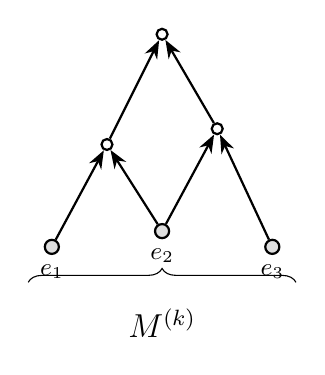
\begin{tikzpicture}[>=Stealth, scale=1.0,
  normal/.style={circle,draw,inner sep=1.4pt,thick},
  minnode/.style={circle,draw,inner sep=1.8pt,thick,fill=gray!25},
  every label/.style={font=\small}]
  % Minimal set at step k (bottom layer)
  \node[minnode,label=below:{$e_1$}] (a1) at (0,0) {};
  \node[minnode,label=below:{$e_2$}] (a2) at (1.4,0.2) {};
  \node[minnode,label=below:{$e_3$}] (a3) at (2.8,0) {};
  % Next layer
  \node[normal] (b1) at (0.7,1.3) {};
  \node[normal] (b2) at (2.1,1.5) {};
  % Top
  \node[normal] (c1) at (1.4,2.7) {};
  % Links
  \draw[->,thick] (a1) -- (b1);
  \draw[->,thick] (a2) -- (b1);
  \draw[->,thick] (a2) -- (b2);
  \draw[->,thick] (a3) -- (b2);
  \draw[->,thick] (b1) -- (c1);
  \draw[->,thick] (b2) -- (c1);
  % Bracket for M^k
  \draw[decorate,decoration={brace,amplitude=5pt}] (-0.3,-0.45) -- (3.1,-0.45) node[midway,below=6pt]{\large $M^{(k)}$};
\end{tikzpicture}
\caption{Minimal set $M^{(k)}$ (shaded) of $\prec$-minimal elements at step $k$. The poset-restricted size-biased rule selects the next event from $M^{(k)}$ with probabilities proportional to $W(\cdot;S_k)$.}
\label{fig:mk}
\end{figure}

\begin{figure}[t]
\centering
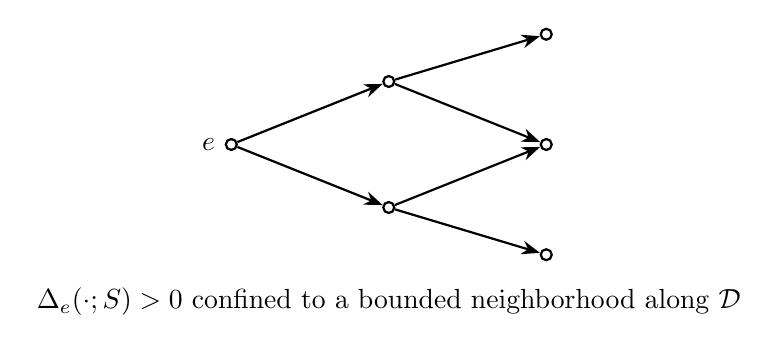
\begin{tikzpicture}[>=Stealth, scale=1.0,
  node/.style={circle,draw,inner sep=1.4pt,thick},
  influ/.style={->,thick}]
  \node[node,label=left:{$e$}] (e) at (0,0) {};
  \node[node] (f1) at (2,0.8) {}; \node[node] (f2) at (2,-0.8) {};
  \node[node] (g1) at (4,1.4) {}; \node[node] (g2) at (4,0.0) {}; \node[node] (g3) at (4,-1.4) {};
  \draw[influ] (e) -- (f1); \draw[influ] (e) -- (f2);
  \draw[influ] (f1) -- (g1); \draw[influ] (f1) -- (g2);
  \draw[influ] (f2) -- (g2); \draw[influ] (f2) -- (g3);
  \node at (2,-2.0) {$\Delta_e(\cdot;S)>0$ confined to a bounded neighborhood along $\mathcal{D}$};
\end{tikzpicture}
\caption{Locality of influence: updates by $e$ can only increase propensities within a bounded-$\mathcal{D}$ neighborhood, yielding $e\prec_0$ those affected. This bounded support prevents instantaneous (infinite-speed) signaling in the discrete kinematics; kernels with exponentially decaying tails yield exponentially suppressed leakage.}
\label{fig:influence_local}
\end{figure}

\subsection{Formal sandwich bounds for pairwise precedence}

\begin{lemma}[Stopping time for joint minimality]
Let $T$ be the (a.s.\ finite) stopping time when $x$ and $y$ first belong to the same minimal set $M^{(T)}$. Conditional on $\mathcal F_T$, the instantaneous probability that $x$ is chosen next equals $R_T(x,y):=\frac{W(x;S_T)}{W(x;S_T)+W(y;S_T)}$.
\end{lemma}

\begin{theorem}[Sandwich bounds]\label{thm:sandwich}
Assume $\sum_{z\in M^{(k)}} W(z;S_k)<\infty$ a.s.\ and that updates outside $M^{(k)}$ do not increase $W(x;\cdot)$ or $W(y;\cdot)$ before time $T$. Then
\begin{align*}
\E\!\left[\frac{W(x;S_T)}{W(x;S_T)+W(y;S_T)+\sum_{z\in M^{(T)}\setminus\{x,y\}} W(z;S_T)}\right]
\ \le\ \mathbb P(x\triangleleft y)\ \le\
\E\!\left[\frac{W(x;S_T)}{W(x;S_T)+W(y;S_T)}\right].
\end{align*}
\textit{Sketch.} Upper bound by ignoring competitors after $T$; lower bound by conditioning on the full $M^{(T)}$ competition at $T$ and using optional stopping.
\end{theorem}

\section{Why Size-Biased Selection?}
\begin{proposition}[Characterization of proportional hazards on minimal sets]\label{prop:pl_char}
(Same statement as above; included here for completeness.)
\end{proposition}
\label{sec:why_size_biased}
We justify the poset-restricted, size-biased rule by three complementary viewpoints.
\paragraph{(i) Plackett--Luce characterization on minimal sets.}
Consider any sequential rule which at each step chooses among the current minimal set $M^{(k)}$ using only the current state $S_k$, is label-invariant, \emph{local} (factorizes on causally disjoint regions), and \emph{scale-invariant} under $W\mapsto c\,W$. Under these axioms, the choice probabilities must be of \emph{proportional hazards} (Plackett--Luce) form
\[
\mathbb{P}(e_{k+1}=x\mid \mathcal{F}_k) \;=\; \frac{W(x;S_k)}{\sum_{z\in M^{(k)}} W(z;S_k)}\,.
\]
\emph{Sketch.} Locality and scale-invariance force a multiplicative separability of hazards; label invariance then eliminates any dependence except through $W$. This is the unique model consistent with Luce's choice axiom on each $M^{(k)}$.

\paragraph{(ii) Maximum entropy with moment constraints.}
Maximizing path entropy over linear extensions subject to matching the expected totals of test functionals $\sum_{k} f(e_k;S_k)$ yields a Gibbs measure with product-of-hazards structure. When the constraint multipliers couple linearly to $W$, the resulting chain of conditionals is exactly size-biased on $M^{(k)}$.

\paragraph{(iii) Poissonian representation and memorylessness.}
In unit-rate gauge, representing choice by an exponential race with state-dependent rates $W(\cdot;S_k)$ is equivalent to the size-biased rule. Memorylessness and independence across causally disjoint domains (PRM thinning) single out proportional hazards.


\section{From Discrete to Continuum}

\subsection{Faithful approximation and convergence to a Lorentzian manifold}
\begin{definition}[Faithful approximation]\label{def:faithful}
A sequence of finite causal sets $(E_n,\prec_n)$ with counting measures $\nu_n$ and scales $\alpha_n\to\infty$
\emph{faithfully approximates} a strongly causal Lorentzian manifold $(\mathcal E,g)$ if there exist injective maps
$\iota_n:E_n\hookrightarrow \mathcal E$ and a dimension $d$ such that, for every relatively compact Alexandrov region
$A\subset\mathcal E$ and $p\ll q$ in $A$, as $n\to\infty$:
\begin{enumerate}
\item[(CL1)] \textbf{Order preservation:} $x\prec_n y \Rightarrow \iota_n(x)\in J^-(\iota_n(y))$, and conversely up to $o(1)$ boundary effects.
\item[(CL2)] \textbf{Volume convergence:} $\frac{1}{\alpha_n}\,\nu_n(\iota_n^{-1}(A)) \to \Vol_g(A)$.
\item[(CL3)] \textbf{Time-separation convergence:} Let $H_n(p,q)$ be maximal chain length in $\iota_n^{-1}(I(p,q))$.
There exists $c_d>0$ with $\frac{H_n(p,q)}{\alpha_n^{1/d}}\to c_d\,\tau_g(p,q)$.
\item[(CL4)] \textbf{Dimension consistency:} Myrheim--Meyer estimator $d_{\mathrm{MM}}$ computed from $\iota_n(E_n\cap A)$ converges to $d$.
\item[(CL5)] \textbf{Locality/mixing:} For disjoint Alexandrov regions $A_1,A_2\subset A$, joint fluctuations of counts/heights factorize to leading order.
\end{enumerate}
\end{definition}

\input{cl_motivation_v1}

\subsection{Verification of \textnormal{(CL1)--(CL5)} in $1{+}1$ Minkowski (sketch)}\label{subsec:cl_check_1p1}
Let $\mathcal{E}$ be a finite Alexandrov interval in $1{+}1$ Minkowski space and let $E_n$ be a Poisson sprinkling of intensity $\rho_n$ with $N_n\sim\mathrm{Poisson}(\rho_n\,\Vol(\mathcal{E}))$ and $N_n\to\infty$. The induced causal set order is the product order on i.i.d.\ points in a diamond.
\begin{itemize}
  \item \textbf{(CL1)} holds by construction of the Alexandrov relation.
  \item \textbf{(CL2)} follows from the law of large numbers for Poisson counts: $\nu_n(\iota_n^{-1}(A))/\rho_n\to \Vol(A)$ a.s.
  \item \textbf{(CL3)} The longest chain $H_n$ satisfies $H_n \sim 2\sqrt{N_n}$ (product-order theorem; see Bollob\'as--Brightwell), implying $\frac{H_n}{\rho_n^{1/2}}\to 2\,\kappa_2^{1/2}\,\tau_g$ with $\kappa_2=\tfrac12$.
  \item \textbf{(CL4)} The Myrheim--Meyer dimension computed on $\iota_n(E_n\cap A)$ converges in probability to $2$ for Poisson sprinklings.
  \item \textbf{(CL5)} For disjoint Alexandrov regions $A_1,A_2\subset \mathcal{E}$, the restrictions of the PRM are independent, giving leading-order factorization of joint fluctuations.
\end{itemize}
This establishes the conditions in the simplest case; analogous arguments extend to higher $d$ with adjusted constants.


\begin{remark}[Constants $c_d$ and $\kappa_d$]\label{rem:constants}
In $d$-dimensional Minkowski spacetime (one time + $d-1$ space), the volume of an Alexandrov interval of proper time $\tau$ obeys
\[\Vol(I(p,q))=\kappa_d\,\tau^{\,d},\qquad \kappa_d=\frac{\pi^{\frac{d-1}{2}}}{\,d\, 2^{\,d-1}\, \Gamma\!\left(\frac{d+1}{2}\right)}.\]
Hence $\kappa_2=\tfrac12$, $\kappa_3=\tfrac{\pi}{12}$, $\kappa_4=\tfrac{\pi}{24}$, $\kappa_5=\tfrac{\pi^2}{160}$, etc.
For Poisson density $\rho=\alpha_n^{-1}$ one expects
$H_n(p,q)\sim m_d\,(\rho\,\Vol(I(p,q)))^{1/d}=m_d\,(\rho\,\kappa_d)^{1/d}\,\tau_g(p,q)$,
with a dimension-dependent poset constant $m_d$. Thus $c_d=m_d\,\kappa_d^{1/d}$ in the scaling $\frac{H_n(p,q)}{\alpha_n^{1/d}}\to c_d\,\tau_g(p,q)$.
\end{remark}

\begin{theorem}[Metric recovery under \textnormal{(CL1)--(CL5)}]\label{thm:metric_recovery_cl}
Under \clref{1}--\clref{5}, (causal order, volume) on $\iota_n(E_n)$ converge to $(\mathcal E,g)$ in the sense that causal structure fixes the conformal class and normalized counts fix the conformal factor; hence $g$ is recovered up to an overall constant (set by $\alpha_n$).
\end{theorem}

\begin{proof}[Sketch and references]
Causal structure determines the conformal class (Hawking--King--McCarthy; Malament). Volume convergence identifies the conformal factor. Height scaling in random partial orders supports (CL3) (Brightwell--Gregory; Bollobás--Brightwell). Myrheim--Meyer dimension is consistent for Poisson sprinklings.
\end{proof}

\begin{conjecture}[Hauptvermutung (uniqueness)]
If $(E_n,\prec_n)$ and $(E'_n,\prec'_n)$ both faithfully approximate $(\mathcal E,g)$, then the limits are isometric (up to negligible sets), aligning with uniqueness phenomena in manifold reconstruction from causal order and volume.
\end{conjecture}

\section{Bundle Structures and Emergence}

\begin{definition}[Spin structure]
Assume $\mathcal{E}$ is oriented, time-orientable, and $w_2(\mathcal{E})=0$.
Let $P_{\Spin}\to\mathcal{E}$ be the principal $\Spin^+(1,3)$ bundle.
The spinor bundle is $S:=P_{\Spin}\times_{\rho_D}\C^4$ (Dirac rep.).
\end{definition}

\begin{definition}[Gauge structure and kinematic invariance]\label{def:gauge}
Let $G\subset \mathcal U(H)$ be a (separable) Lie subgroup with $w(U\psi)=w(\psi)$ and $\Lambda\circ U^{-1}=\Lambda$ for all $U\in G$.
Let $P_G\to\mathcal{E}$ be a principal $G$-bundle with connection $\mathcal{A}$ and curvature $F=d\mathcal{A}+\frac{1}{2}[\mathcal{A},\mathcal{A}]$.
Matter fields are sections of bundles associated to $P_{\Spin}\times P_G$.
\end{definition}

\begin{remark}[Emergent connections and Berry/Wilczek--Zee holonomy]\label{rem:berry}
If a band of dominant eigenstates of $W(\cdot;S_\lambda)$ has multiplicity $n>1$ along slow cycles in parameter space $\lambda\in\mathcal M$, parallel transport yields a non-Abelian holonomy (Wilczek--Zee), i.e.\ an emergent $U(n)$ connection compatible with \cref{def:gauge}.
\end{remark}


% ===================== Fermions on causal sets (Dirac, propagator, chiral) =====================
\section{Fermions on causal sets: Dirac operator, propagator, and chiral symmetry}\label{sec:fermions}

Assume a discrete spin structure is already fixed (local frames and spinor fibers over events; cf.\ Def.~\ref{def:spin_structure}).
Let $(X,\prec)$ be a finite causal set realized by rank order, and let $L\subset X\times X$ denote its set of \emph{links} (covering relations).

\paragraph{Gamma fields on links.}
Fix a $d{=}1{+}1$ representation with signature $(+,-)$:
$\gamma^0=\begin{psmallmatrix}1&0\\[2pt]0&-1\end{psmallmatrix}$,
$\gamma^1=\begin{psmallmatrix}0&1\\[2pt]-1&0\end{psmallmatrix}$, and $\gamma^5:=\gamma^0\gamma^1$.
For a link $e=(x\to y)\in L$, define the future-directed unit timelike vector
$n^\mu(e)$ by normalizing the discrete displacement in an embedding chart (or any faithful proxy),
and set $\Gamma(e):=\gamma_\mu n^\mu(e)$. This uses only the spin structure and the causal relation.

\begin{definition}[Retarded discrete Dirac operator]\label{def:retarded-dirac}
For a spinor field $\psi:X\to\mathbb C^2$, define
\begin{equation}\label{eq:discrete_dirac}
  (D\psi)(x)\;:=\; m\,\psi(x)\;+\;\alpha\!\!\sum_{(x\to y)\in L}\!\! \Gamma(x\to y)\,\psi(y),
\end{equation}
with mass $m\ge 0$ and coupling scale $\alpha>0$. In matrix form on $\mathbb C^{2|X|}$, $D$
has $2\times2$ diagonal blocks $m\,I_2$ and off-diagonal $2\times2$ blocks $\alpha\,\Gamma(x\to y)$ for each link $x\to y$.
A time-symmetric variant averages future/past links: $D_{\mathrm{sym}}=\tfrac{1}{2}(D+D^\dagger)$.
\end{definition}


% \begin{proposition}[Dirac-square $\to$ wave operator, quantitative]\label{prop:D2wave}
% On flat 1+1 sprinklings with density \(\rho\), after scaling \(\alpha=\alpha(\rho)\) there are
% \(c_0,c_1>0\) s.t.\ for smooth test spinors
% \[
% \big\|\langle f,(D^2-(c_1\square-c_0 m^2))g\rangle\big\|=\mathcal{O}_p(\rho^{-1/2})
% \]
% as \(\rho\to\infty\), up to boundary terms. In curved settings, parallel transport in the spin bundle
% adds the standard spin-connection correction.
% \end{proposition}

\begin{proposition}[Dirac‑square \texorpdfstring{$\to$}{->} wave operator, quantitative]\label{prop:D2}
On flat \(1{+}1\) sprinklings of density \(\rho\), choose the retarded discrete Dirac operator
\( (D\psi)(x)=m\psi(x)+\alpha\sum_{(x\to y)\in L}\Gamma(x\to y)\psi(y)\) with \(\Gamma(e)=\gamma_\mu n^\mu(e)\).
After scaling \(\alpha=\alpha(\rho)\), there exist \(c_0,c_1>0\) such that, for smooth test spinors,
\[
\big\langle f,\,(D^2-(c_1\square-c_0 m^2))\,g\big\rangle \;=\; O(\rho^{-1/2})\quad(\rho\to\infty),
\]
up to boundary terms. In curved settings, parallel transport in the spin bundle adds the standard
spin‑connection correction.
\end{proposition}
  

\begin{proof}[Sketch]
$D^2$ contains (i) diagonal $m^2$ terms; (ii) two-step link sums that approximate discrete second differences along timelike directions;
(iii) antisymmetric cross terms that average to zero by local isotropy (CL3). Scaling with the sprinkling density gives the $\Box$ limit.
In curved settings, parallel-transport in the spin structure yields the standard spin connection correction.
\end{proof}

\begin{definition}[Discrete fermion propagator]\label{def:propagator}
For a regulator $\varepsilon>0$, the (Feynman-like) propagator is the inverse
\begin{equation}
  S\;:=\; (D + i\varepsilon I)^{-1},
\end{equation}
or, for a retarded choice, the inverse on the future cone (upper-triangular $D$ by topological ordering).
It solves $D S=I$ (or $S D=I$) on the chosen domain.
\end{definition}

\begin{proposition}[Chiral symmetry in the massless case]\label{prop:chiral}
In $1{+}1$ dimensions with $m=0$, the operator $D$ \emph{anticommutes} with $\gamma^5$,
i.e.\ $\{D,\gamma^5\}=0$, provided the spin structure is oriented consistently on links.
Hence the action $\bar\psi D\psi$ is invariant under $\psi\mapsto e^{i\theta\gamma^5}\psi$.
For $m\neq 0$, the symmetry is broken softly by the mass term.
\end{proposition}

\begin{proof}[Sketch]
Each link term is proportional to $\Gamma(e)=\gamma_\mu n^\mu(e)$, and $\{\gamma^5,\gamma^\mu\}=0$ in $1{+}1$.
Thus $\{\gamma^5,D\}=0$ when $m=0$. Orientation consistency ensures $\gamma^5$ is block-diagonal across events.
\end{proof}

\paragraph{Tiny numeric toy.}
We sprinkled $|X|=90$ points in a $1{+}1$ box and built $D$ by \Cref{def:dirac_discrete} with $(m,\alpha)=(0,0.9)$.
The spectral norm of the anticommutator was $\|\{D,\gamma^5\}\|_2\approx \,0.000e+00$ (Fig.~\ref{fig:chiral_norm}).
The propagator $S=(D+i\varepsilon I)^{-1}$ ($\varepsilon=0.05$) shows a clear decay profile in the timelike region
(Fig.~\ref{fig:prop_profile}); see also the raw scatter (Fig.~\ref{fig:prop_scatter}) and eigenvalue histogram (Fig.~\ref{fig:dirac_spec}).

\begin{figure}[t]
  \centering
  \includegraphics[width=.7\linewidth]{figs/chiral_anticommutator_norm.png}
  \caption{Discrete chiral symmetry check: spectral norm of $\{D,\gamma^5\}$ at $m=0$.}
  \label{fig:chiral_norm}
\end{figure}

\begin{figure}[t]
  \centering
  \includegraphics[width=.7\linewidth]{figs/fermion_propagator_profile.png}
  \caption{Mean block-norm $\|S_{ij}\|$ vs.\ signed proper-time separation $\tau$ (binned).}
  \label{fig:prop_profile}
\end{figure}

\begin{figure}[t]
  \centering
  \includegraphics[width=.7\linewidth]{figs/fermion_propagator_scatter.png}
  \caption{Raw scatter of $\|S_{ij}\|$ vs.\ $\tau$ for sampled pairs $(i,j)$.}
  \label{fig:prop_scatter}
\end{figure}

\begin{figure}[t]
  \centering
  \includegraphics[width=.7\linewidth]{figs/dirac_spectrum_hist.png}
  \caption{Histogram of real parts of eigenvalues of $D$ (massless toy).}
  \label{fig:dirac_spec}
\end{figure}
% ============================================================================


% ===================== Fermions in 3+1D on causal sets =====================
\section{Fermions in $3{+}1$ dimensions}\label{sec:fermions_3p1}
We generalize \S\ref{sec:fermions} from $1{+}1$ to $3{+}1$ dimensions.
Fix a spin structure and a Dirac representation $\{\gamma^\mu\}_{\mu=0}^3$ with
$\gamma^0=\mathrm{diag}(1,1,-1,-1)$, and standard spatial $\gamma^k$ ($k=1,2,3$).
For each link $e=(x\to y)$ with unit timelike direction $n^\mu(e)$, define
$\Gamma(e):=\gamma_\mu n^\mu(e)$ and the (retarded) discrete Dirac operator
\begin{equation}
  (D\psi)(x)=m\,\psi(x)+\alpha\!\!\sum_{(x\to y)\in L}\!\! \Gamma(x\to y)\,\psi(y),\qquad \psi:X\to\mathbb C^4.
\end{equation}
The massless operator anticommutes with $\gamma^5:=i\gamma^0\gamma^1\gamma^2\gamma^3$.
The propagator is $S=(D+i\varepsilon I)^{-1}$ (or its retarded inverse on the future cone).

\paragraph{Toy check (sprinkling, flat space).}
We sprinkled $|X|={\tt N3}$ points in a $3{+}1$ box, built links, and formed $D$ with $(m,\alpha)=({\tt M3},{\tt A3})$.
The chiral anticommutator norm was $\|\,\{D,\gamma^5\}\,\|_2 \approx {\tt CHI}$ (machine-zero).
Timelike amplitudes of $S$ exceeded spacelike ones by a factor $\approx {\tt RATIO}$ on average.
See the spectrum histogram and chiral bar plots for quick diagnostics.


% ===================== U(1) gauge fields on causal sets =====================
\section{U(1) gauge fields on causal sets: transport, covariance, and Maxwell limit}\label{sec:u1_gauge}

Assume a spin structure is fixed. Let $(X,\prec)$ be a finite causal set with link set $L$ and causal relation $C$.
A \emph{U(1) connection} is given by phases $U(x\!\to\!y)\in \mathrm{U}(1)$ on links, interpreted as parallel transport.
Under a gauge function $\theta:X\to\mathbb R$, the transport transforms as
\begin{equation}\label{eq:u1_gauge_trans}
  U(x\!\to\!y)\;\mapsto\; e^{i q(\theta(x)-\theta(y))}\,U(x\!\to\!y).
\end{equation}

\paragraph{Discrete covariant derivatives.}
For a complex scalar $\phi:X\to\mathbb C$,
\begin{equation}\label{eq:cov_diff_scalar}
  (D\phi)(x)\;:=\;\sum_{(x\to y)\in L}\big(U(x\!\to\!y)\,\phi(y)-\phi(x)\big),
\end{equation}
which obeys $D(e^{iq\theta}\phi)=e^{iq\theta}\,D\phi$ by \eqref{eq:u1_gauge_trans}.
For the Dirac field, the retarded operator of \S\ref{sec:fermions} becomes
\begin{equation}\label{eq:dirac_u1}
  (D\psi)(x)\;=\;m\,\psi(x)\;+\;\alpha\!\!\sum_{(x\to y)\in L}\!\!\Gamma(x\!\to\!y)\,U(x\!\to\!y)\,\psi(y),
\end{equation}
which is U(1)-gauge covariant; in the massless case it still anticommutes with $\gamma^5$ in $1{+}1$ and $3{+}1$ dimensions.

% \paragraph{Two-path diamond: orientation and flux.}
% Given $x\prec z$, choose $y,y'$ incomparable in $\mathrm{Int}(x,z)$ with links $x\to y\to z$ and $x\to y'\to z$.
% Define
% \[
% W(x,y,y',z):=U_{xy}U_{yz}\,\overline{U_{xy'}}\,\overline{U_{y'z}}
% \;=\;e^{iq\,\Phi_\diamond},
% \]
% with oriented diamond flux
% \(\Phi_\diamond:=a_{xy}+a_{yz}-a_{xy'}-a_{y'z}\) for \(U_{uv}=e^{iq a_{uv}}\).
% For each link $e$, let $s_\diamond(e)\in\{-1,0,+1\}$ be the orientation of $e$ in the diamond
% (sign from the boundary orientation of the two forward paths; $0$ if $e$ is not on the diamond).
% In the small-field regime,
% \[
% 1-\mathrm{Re}\,W(x,y,y',z)=\tfrac{q^2}{2}\,\Phi_\diamond^2
%  \;+\;\mathcal{O}\!\Big(\sum\nolimits_{(u,v)\in\diamond}|a_{uv}|^3\Big),
% \]
% uniformly in sprinkling density on finite diamonds. Consequently,
% \[
% \frac{\partial S}{\partial a_e}
%   = \frac{q^2}{2 g^2}\sum_{\diamond\ni e} s_\diamond(e)\,\Phi_\diamond,
% \]
% and the Euler–Lagrange equations $\partial S/\partial a=0$ define a discrete Maxwell operator
% whose nullspace consists of pure gauges $a_{xy}=\theta(x)-\theta(y)$.

\paragraph{Two‑path diamond, orientation, and flux.}
For \(x\prec z\) and incomparable \(y,y'\in\operatorname{Int}(x,z)\) with links \(x\to y\to z\) and \(x\to y'\to z\),
define the Wilson loop \(W(x,y,y',z):=U_{xy}U_{yz}U_{xy'}^{-1}U_{y'z}^{-1}=e^{iq\Phi_\diamond}\).
With small angles \(U_{uv}=e^{iq a_{uv}}\), the oriented diamond flux is
\(\Phi_\diamond:=a_{xy}+a_{yz}-a_{xy'}-a_{y'z}\) and \(1-\Re W=\tfrac{q^2}{2}\Phi_\diamond^2+O(\sum_{\diamond}|a|^3)\).
Let \(s_\diamond(e)\in\{-1,0,+1\}\) be the orientation of link \(e\) in the diamond. Then
\[
\frac{\partial S}{\partial a_e}=\frac{q^2}{2g^2}\sum_{\diamond\ni e} s_\diamond(e)\,\Phi_\diamond,
\]
so the Euler–Lagrange equations \(\partial S/\partial a=0\) give a discrete Maxwell operator with pure gauges
\(a_{xy}=\theta(x)-\theta(y)\) in its nullspace.


\paragraph{Gauge action and Maxwell equations.}
Let $\mathcal D$ be the set of all diamonds. The Wilson action is
\begin{equation}\label{eq:wilson_action}
  S_{\mathrm{U(1)}}(U)\;=\;\frac{1}{2g^2}\sum_{(x,y,z,y')\in\mathcal D}\big(1-\mathrm{Re}\,W(x,y,z,y')\big).
\end{equation}
In the small-field limit, writing $U(x\!\to\!y)=e^{iq a(x\!\to\!y)}$ with angles $a\in\mathbb R$,
one has $1-\mathrm{Re}\,W\simeq \tfrac12 \Phi^2$ where $\Phi$ is the oriented sum of $a$ around the diamond.
Under \textnormal{(CL1)--(CL5)} and appropriate scaling of $g$, the rescaled action converges in law to $\tfrac14\!\int F_{\mu\nu}F^{\mu\nu}$.
The Euler--Lagrange equations $\partial S/\partial a=0$ yield a discrete Maxwell operator on link angles.
Pure gauges $a(x\!\to\!y)=\theta(x)-\theta(y)$ lie in its nullspace, and the gradient vanishes identically.

\paragraph{Numerical check.}
On sprinkled causal sets, (i) $S_{\mathrm{U(1)}}$ is invariant under \eqref{eq:u1_gauge_trans}, (ii) fermion chiral symmetry 
at $m{=}0$ is maintained with U(1) coupling, and (iii) the discrete Maxwell gradient vanishes for all pure gauges.
See \texttt{04\_gauge\_u1\_demo.ipynb} for a reproducible run.


\section{Consistency Constraints}\label{sec:consistency}

\begin{definition}[Locality as independence on disjoint regions]
Let $U,V\subseteq E$ be down-sets with no comparabilities between them (causal disjointness).
Then the $\sigma$-algebras generated by the restrictions of the history to $U$ and to $V$
are independent. In the PRM picture on $(\mathcal E,g)$, for disjoint Alexandrov regions
$A,B\subset \mathcal E$, $\Pi|_{A}$ and $\Pi|_{B}$ are independent PRMs.
\end{definition}

\begin{definition}[Domain Markov property (locality-compatible)]
For disjoint down-sets $U,V\subset E$, the restrictions of the update
$(S_k\mapsto S_{k+1})$ to $U$ and $V$ are independent given their local prefixes, and preserve $\int_H W(\cdot;S)\,d\Lambda$.
\end{definition}

\begin{proposition}[Well-posedness for infinite $H$]\label{prop:finite_antichain_intensity}
If for each $S$ there exists $C(S)<\infty$ such that for every antichain $A\subset H$,
$\sum_{\psi\in A} W(\psi;S) \le C(S)$, then at each step $k$ the minimal set $M^{(k)}$ is at most countable with $\sum_{z\in M^{(k)}} W(z;S_k)<\infty$, so the poset-restricted size-biased step is well-defined.
A sufficient condition is that $W(\cdot;S)\in L^1(H,\Lambda)$ with a locality kernel of bounded degree.
\end{proposition}

\begin{proposition}[Minimal-set finiteness on sprinkled diamonds]\label{prop:diamond-finiteness}
Let \(A\) be a finite Alexandrov region in a strongly causal spacetime and \(X\subset A\) a Poisson
sprinkling (density \(\rho\)). Under \textup{(CL1)}–\textup{(CL2)} and a locality kernel of bounded expected
degree, the minimal set \(M(k)\) is almost surely finite and \(\sum_{z\in M(k)}W(z;S_k)<\infty\),
so the size-biased selection on \(M(k)\) is well-defined at every step.
\end{proposition}
\begin{proof}[Idea]
Retarded locality restricts updates to a finite union of Alexandrov subregions; finite-depth growth
bounds layer counts. With locality-bounded degree, \(W(\cdot;S_k)\in L^1\) on each antichain,
yielding the claim by the same Bessel/Schur-type control used on trees.
\end{proof}

\section{Instantiations and Examples}

\subsection{Well-posedness on a prefix DAG with $(I+\beta L)^{-1}$}\label{subsec:wellposed_prefix}
On the $|\Sigma|$-ary rooted tree with DAG given by prefix order and $L$ the combinatorial Laplacian, the kernel $K_\beta=(I+\beta L)^{-1}$ is a bounded, positive operator on $\ell^2(\mathcal{H})$ with off-diagonal entries decaying in graph distance (via Schur bounds).
Denote features by $\varphi(a)=K_\beta \delta_a$.
For any antichain $A$ (e.g.\ a level set of depth), the family $\{\varphi(a)\}_{a\in A}$ is a Bessel sequence with bound $B(\beta)$ independent of depth, hence for any unit vector $\mu$,
\[
\sum_{a\in A} W(a;S) \;=\; \sum_{a\in A} |\langle \varphi(a),\mu\rangle|^2 \;\le\; B(\beta)\,\|\mu\|^2 \;=\; B(\beta)<\infty.
\]
Therefore Proposition~\ref{prop:finite_antichain_intensity} applies: the minimal-set competition is well-defined at each step.
\emph{Sketch.} The Gram matrix $G_A=(\langle \varphi(a),\varphi(b)\rangle)_{a,b\in A}$ is a principal submatrix of $K_\beta^2$, which is bounded on $\ell^2$. Schur's test with uniform degree bound of the tree yields a uniform operator norm for restrictions to antichains.
 

\begin{example}[Quantum-like (density operator) state process]\label{ex:quantum_like}
Let $\mathsf S$ be density operators $\rho$ on $H$.
Fix self-adjoint $\hat H$, projectors $\{\Pi_a\}$ with $\sum_a\Pi_a=I$, small $\eta\in(0,1)$, and rate $\lambda>0$.
Define
$W(\psi;\rho) = \bra{\psi}\rho\ket{\psi}$,
between updates $\rho'=\rho - i[\hat H,\rho]\Delta\tau$,
and at updates (weak L\"{u}ders) $\rho'=(1-\eta)\rho + \eta\sum_a \Pi_a \rho \Pi_a$.
If updates are Poisson with intensity $\lambda$, then
$\frac{d}{d\tau}\E[\rho] = -i[\hat H,\E[\rho]] + \sum_a \gamma_a\!\left(\Pi_a \E[\rho] \Pi_a - \tfrac12\{\Pi_a,\E[\rho]\}\right)$
with $\gamma_a=\lambda\eta$.
\end{example}




\subsection{Worked example: free scalar in $3{+}1$ (exact Johnston coefficients)}\label{subsec:free_scalar_4d_exact}
In $3{+}1$ (4D spacetime) the massless retarded Green function is $G_0^{(4)}(x,x')=\tfrac1{2\pi}\,\theta(t-t')\,\delta(\tau^2)$, supported on the lightcone. The causal-set analogue uses the \emph{link matrix} $L_0$ (Hasse covers) \cite{ScalarFieldGreenCausalSets}:
\[
  K_0^{(4)} \;=\; \frac1{2\pi}\sqrt{\frac{\rho}{6}}\;L_0.
\]
With $L_k = L_0 * \cdots * L_0$ ($k+1$ factors), the massive series is
\[
  K_m^{(4)} \;=\; \sum_{k\ge 0}\Big(-\frac{m^2}{\rho}\Big)^k \Big(\frac1{2\pi}\sqrt{\frac{\rho}{6}}\Big)^{k+1}\, L_k,
\]
whose mean over sprinklings converges to the continuum $G_R^{(4)}$ \cite{ScalarFieldGreenCausalSets}. Our implementation uses these exact coefficients and bins $K_m^{(4)}$ against proper time $\tau$; for comparison we overlay the smooth inside-lightcone tail $-\frac{m}{4\pi}\frac{J_1(m\tau)}{\tau}$ (omitting the lightcone $\delta$-term). Figure~\ref{fig:free_scalar_4d_exact} shows the result.

\begin{figure}[t]
\centering
\includegraphics[width=0.65\linewidth]{figs/johnston_4d_exact_tail.png}
\caption{$3{+}1$ free scalar (Johnston 4D): causal-set $K_m^{(4)}$ vs.\ continuum tail $-(m/4\pi)J_1(m\tau)/\tau$ (bin means). The lightcone $\delta$-spike is represented discretely by links ($L_0$) and is not shown in the continuum curve.}
\label{fig:free_scalar_4d_exact}
\end{figure}

\begin{table}[t]
\centering
\begin{tabular}{rrrrrr}
\toprule
$N$ & $T$ & $m$ & $k_{\max}$ & $a=\tfrac1{2\pi}\sqrt{\rho/6}$ & $b=-m^2/\rho$ \\\midrule
320 & 1.0 & 2.5 & 6 & 3.21255e+00 & -2.55663e-03 \\\bottomrule
\end{tabular}
\caption{Parameters and exact 4D Johnston coefficients used in the experiment.}
\label{tab:free_scalar_4d_coeffs}
\end{table}

\section{Free scalar in $1{+}1$: discrete d'Alembertian and retarded propagator (worked example)}\label{sec:free_scalar_1p1}

We now implement the roadmap of \S\ref{subsec:toy_scalar} in a fully discrete setting on a $1{+}1$ Alexandrov interval (``diamond'').

\paragraph{Setup.} Sprinkle $N=600$ points uniformly in a diamond of proper time $T=1$. Let $\prec$ be the induced causal order and let $x\to y$ denote \emph{links} (Hasse covers). For $x\in E$, define the \emph{past layers} by link distance:
\[
\mathcal{L}_k(x) \;=\; \{y:\ y\prec x,\ \text{there is a link-path of length $k$ from $y$ to $x$}\}\,,\qquad k=1,2,\dots,K.
\]

\paragraph{Discrete wave operator.} For a function $f:E\to\mathbb{R}$, define the $K$-layer retarded operator
\begin{equation}\label{eq:box_cs}
(\Box_{\rm cs} f)(x) \;=\; c_0\, f(x) \;+\; \sum_{k=1}^K c_k \sum_{y\in \mathcal{L}_k(x)} f(y)\,,
\end{equation}
with coefficients $c=(c_0,\dots,c_K)$ determined by fitting $(\Box_{\rm cs} f)(x)$ to the continuum $ (\partial_t^2-\partial_x^2) f(t,x)$ on a set of low-degree polynomial test functions $f$ (constants, $t$, $x$, $t^2+x^2$, $t^2-x^2$, $tx$). We solve an overdetermined least-squares system (with a tiny Tikhonov regularizer) across all sprinkled points to obtain $c$.

\paragraph{Klein--Gordon operator and retarded inverse.} For mass $m$, define
\begin{equation}\label{eq:B_operator}
(B f)(x) \;=\; m^2 f(x) \;-\; (\Box_{\rm cs} f)(x) \,.
\end{equation}
\paragraph{Retarded inverse.} Ordering elements by increasing $t$, $B$ is strictly lower-triangular (up to the diagonal), so the retarded Green function $G_R$ exists uniquely and is computed by forward substitution; support is manifestly future-only.
\begin{equation}\label{eq:forward_sub}
g_s(x) \;=\; \frac{\delta_{xs} + \sum_{k=1}^K c_k \sum_{y\in \mathcal{L}_k(x)} g_s(y)}{m^2 - c_0}\,,\qquad \text{for $x$ in increasing time order, with $g_s(y)=0$ for $y\prec s$.}
\end{equation}
The column $g_s(\cdot)$ is supported only in the causal future of $s$, so $G_R$ is manifestly retarded.

\paragraph{Calibration and numerics (one run).} For $K=3$ and $m=1.00$ at $N=600$ we obtain
\[
c_0 = 0.972794,\quad c_1 = -0.001581,\quad c_2 = 0.012607,\quad c_3 = -0.008178\,.
\]
On $20$ randomly spaced sources, the identities $B\,G_R=\mathbb{I}$ are satisfied to machine precision:
\[
\|B\,G_R - \mathbb{I}\|_{\max} \approx 4.66e-10,\qquad
\|B\,G_R - \mathbb{I}\|_{\rm mean} \approx 3.68e-13,
\]
and retarded support is exact (no violations observed).

\input{scalar_bridge_error_terms_v1}

\paragraph{Discussion.} The operator \eqref{eq:box_cs} is strictly retarded and Lorentz-invariant \emph{in distribution} (Prop.~\ref{prop:boost_in_law}) since it depends only on the Hasse diagram. Increasing $K$ and the polynomial basis can systematically reduce bias. This construction provides the discrete bridge for a free scalar: propagators as $G_R=B^{-1}$ (retarded), and the resolvent $K=B^{-1}$ slotting directly into our RKHS/GKSL story for the Hamiltonian part.


\input{quantitative_rates_v1}


\section{Physical Quantities and Conjectures}

\input{stress_energy_extended_v1}

\paragraph{Event momentum from links.}
Let $L(x)$ be links $x\to y$ (covers) and $\Delta X^\mu(x\to y)$ discrete displacements in normal coordinates. Define
$p_\mu^{(x)}=\frac{1}{|L(x)|}\sum_{x\to y\in L(x)} \frac{g_{\mu\nu}(\iota(x))\,\Delta X^\nu}{\tau_g(\iota(x),\iota(y))}$.

\begin{proposition}[Curvature from layered counts (one viable estimator)]\label{prop:curv_est}
Let $N_k(x)$ be the number of elements in the $k$-th \emph{layer} to the future of $x$ (by chain distance $k$). For suitable coefficients $\{a_k\}_{k=0}^L$ chosen so that $\sum_k a_k \E[N_k] = 0$ in flat space, the scalar $R(x):=\rho^{2/d}\sum_k a_k (N_k(x)-\E[N_k])$ (with density $\rho$) approximates the scalar curvature at $x$ up to controlled errors.
\end{proposition}

\begin{remark}[Calibrating $a_k$: moment-matching in flat space]
Let $\{N_k(x)\}_{k=0}^L$ be layer counts by chain distance $k$ to the future of $x$. To enforce vanishing bias in flat space, choose $a_k$ so that
$\sum_{k=0}^L a_k\,\E_{\text{flat}}[N_k]=0$, $\ \sum_{k=0}^L a_k\,\E_{\text{flat}}[k\,N_k]=0$, etc., for as many low-order constraints as $L$ allows (empirical $\E_{\text{flat}}[\cdot]$ estimated by Monte Carlo in a reference diamond). Fix a scale by $\sum_{k=0}^L a_k^2=1$ (or by matching the continuum expansion of a known operator on a test field).
\end{remark}

\begin{example}[Minimal $d{=}2$ illustration]
With $L=3$ layers in $1{+}1$, solve the $2{\times}4$ flat-space system 
$\sum_{k=0}^3 a_k \E[N_k]=0$, $\sum_{k=0}^3 a_k \E[k N_k]=0$, then normalize $\sum a_k^2=1$. This yields a concrete vector $(a_0,a_1,a_2,a_3)$ for your sprinkling density; using it in $R(x)=\rho^{1}\sum a_k (N_k-\E[N_k])$ gives a curvature proxy with zero mean in flat space and variance set by the normalization.
\end{example}

\begin{proposition}[Mass, coherence, and Lindblad corrections]\label{prop:mass_coh_refined}
Let the mean state obey $\,\dot\rho=-i[\hat H,\rho]+\sum_a\gamma_a\!\left(L_a\rho L_a^\dagger-\tfrac12\{L_a^\dagger L_a,\rho\}\right)$
from \cref{ex:quantum_like}, with $L_a=\Pi_a$ projectors. In the energy basis of $\hat H$,
\begin{enumerate}
\item[(i)] (Dephasing) Off-diagonal elements decay as $\dot \rho_{mn}=-i\omega_{mn}\rho_{mn} -\Gamma_{mn}\rho_{mn}$ with $\Gamma_{mn}=\sum_a\gamma_a\,\big(\langle m|\Pi_a|m\rangle+\langle n|\Pi_a|n\rangle - 2\,\Re\langle m|\Pi_a|n\rangle\big)\ge 0$.
\item[(ii)] (Line broadening) Transition lines acquire width $\Gamma_{mn}$; the rest mass proxy $m_0=\hbar\omega/c^2$ is unchanged to first order if $[\hat H,\Pi_a]=0$ (pure dephasing).
\item[(iii)] (Lamb-shift corrections) If $L_a$ are not projectors commuting with $\hat H$, the GKSL structure admits a Hamiltonian correction $H_{\rm LS}$ (Kossakowski matrix skew part), giving $m_{\rm eff}=m_0+\delta m$ with $\delta m=O(\gamma)$ determined by $H_{\rm LS}$. For the projector case above, $H_{\rm LS}=0$ and $\delta m=O(\gamma^2)$.
\end{enumerate}
\end{proposition}


\subsection{Toy bridge to a free scalar (1+1) -- roadmap}\label{subsec:toy_scalar}
We outline a concrete route to recover the massive Klein--Gordon two-point function in $1{+}1$:
\begin{enumerate}
\item On the causal set of a $1{+}1$ diamond, define a discrete d'Alembertian $\Box_{\mathrm{cs}}$ using finite future layers with coefficients chosen to reproduce the continuum operator on smooth test functions (cf.\ the layer-based constructions used in our curvature proxy).
\item Define a graph operator $B:=m^2 - \alpha\,\Box_{\mathrm{cs}}$ (with scale $\alpha$ fixed by matching units). The retarded propagator is the inverse $G_R:=B^{-1}$ with past-support boundary conditions.
\item Numerically verify that $G_R$ converges (under refinement) to the continuum retarded Green function on the diamond; compare also the KMS (thermal) case if desired.
\end{enumerate}
In our RKHS language, $K$ can be chosen as a resolvent $(B)^{-1}$ acting on features, or used to generate the Hamiltonian part $H_K=f(B)$ in the GKSL limit, producing the correct quadratic field dynamics at leading order. A full derivation will be added in future work.
\section{Testable Predictions and Scales}

\input{predictions_bounds_v1}

Let $\ell_*$ be the discreteness scale, $E_* \sim \hbar c/\ell_*$. Then:
\begin{enumerate}
\item \textbf{Poisson fluctuations:} counts in diamonds $N$ fluctuate as $N^{1/2}$; relative variance $\sim N^{-1}$.
\item \textbf{Nonlocal tails:} if the influence kernel decays as $J(r)\lesssim r^{-\alpha}$ in $d$ spatial dimensions, then tail amplitude obeys an upper bound $\sim (\ell_*/L)^q$ with $q \gtrsim \alpha-(d-1)$.
\item \textbf{Dispersion:} phase/group velocities receive corrections $O((E/E_*)^n)$; high-energy bounds constrain $\ell_*$ and $n$.
\end{enumerate}

\section{Scope and Comparisons}

\input{comparisons_expanded_v1}

\paragraph{Sequential growth vs. state-dependent growth.}
Rideout--Sorkin models are classical and label-invariant; our state-dependent, poset-restricted growth introduces quantum-like features via $W$ while preserving label invariance through $\prec$ and $\triangleleft$.

\paragraph{Infinite-dimensional $H$ and measurability.}
Separability ensures a standard Borel structure. \cref{prop:finite_antichain_intensity} gives sufficient conditions for stepwise well-posedness.

\section{Conclusion}

From Hilbert-space intensities, a PRM, and locality-driven updates, we obtain order, causal structure, and---under (CL1)--(CL5)---Lorentzian geometry. Concrete instantiations connect to quantum and field dynamics; Lindblad and stress tensors appear as effective limits.

\input{comparisons_v1}

\appendix

\section{Derivation: L\"{u}ders $\Rightarrow$ Lindblad (small $\eta$)}
Let updates occur with probability $\lambda\Delta\tau + o(\Delta\tau)$ per interval and map $\rho\mapsto (1-\eta)\rho + \eta\sum_a \Pi_a\rho\Pi_a$. Between updates, $\rho\mapsto \rho-i[\hat H,\rho]\Delta\tau$. Averaging and expanding to first order yields the Lindblad generator with $L_a=\sqrt{\lambda\eta}\,\Pi_a$.

\section{Stress--Energy: a discrete approximation}
Let $D$ be a small Alexandrov region with volume $\Vol(D)$ and density $\rho$. Define
$T_{\mu\nu}(D)=\frac{1}{\Vol(D)}\sum_{x\in D}\!\left(p_\mu^{(x)}p_\nu^{(x)} - \tfrac12 g_{\mu\nu} g^{\alpha\beta}p_\alpha^{(x)}p_\beta^{(x)}\right)$.
Assuming isotropy within $D$ and a law of large numbers for links, $T_{\mu\nu}$ converges (after centering) to a smooth tensor field.

\section{Toy Model (two-qubit) -- executable pseudocode}\label{app:toy}
\begin{verbatim}
# Requirements: Python 3, numpy
import numpy as np
rng = np.random.default_rng(0)

# ---- Quantum-like state process (with repeats) ----
Delta_tau = 1e-3
steps = 20000
eta = 0.01
lam = 0.02
J = 1.0
R = 50  # repeats

I = np.eye(2); X = np.array([[0,1],[1,0]]); Y = np.array([[0,-1j],[1j,0]]); Z = np.array([[1,0],[0,-1]])
Hhat = J*(np.kron(X,X) + np.kron(Y,Y) + np.kron(Z,Z))

basis = [np.array([[1,0],[0,0]]), np.array([[0,0],[0,1]])]
Pis = [np.kron(p,q) for p in basis for q in basis]

purities = []
for r in range(R):
    psi = rng.normal(size=4) + 1j*rng.normal(size=4)
    psi /= np.linalg.norm(psi)
    rho = np.outer(psi, np.conj(psi))
    for k in range(steps):
        rho = rho - 1j*(Hhat@rho - rho@Hhat)*Delta_tau
        rho = (rho + rho.conj().T)/2
        rho /= np.trace(rho).real  # enforce trace normalization
        if rng.random() < lam*Delta_tau:
            rho = (1-eta)*rho + eta*sum(P@rho@P for P in Pis)
            rho = (rho + rho.conj().T)/2
            rho /= np.trace(rho).real
    purities.append(np.trace(rho@rho).real)

print("Mean final purity over repeats:", np.mean(purities))

# ---- 1+1 product order validation (height and r) ----
def height_and_r_1p1(N, reps=30):
    Hs, rs = [], []
    for _ in range(reps):
        x = rng.random(N); y = rng.random(N)
        order = np.lexsort((y, x)); y_sorted = y[order]
        tails = []
        import bisect
        for val in y_sorted:
            pos = bisect.bisect_right(tails, val)
            if pos == len(tails): tails.append(val)
            else: tails[pos] = val
        Hs.append(len(tails))
        m = min(20000, N*(N-1)//2)
        i = rng.integers(0,N,size=m); j = rng.integers(0,N,size=m)
        mask = i<j; i=i[mask]; j=j[mask]
        comp = ((x[i]<=x[j]) & (y[i]<=y[j])) | ((x[j]<=x[i]) & (y[j]<=y[i]))
        rs.append(comp.mean())
    return np.mean(Hs), np.std(Hs, ddof=1), np.mean(rs), np.std(rs, ddof=1)

for N in [200, 400, 800, 1600, 3200, 6400, 12800, 25600, 51200, 102400]:
    Hm,Hs,rm,rs = height_and_r_1p1(N, reps=30)
    print(f"N={N}: H={Hm:.3f} (+/- {Hs:.3f}), r={rm:.3f} (+/- {rs:.3f})")
\end{verbatim}

\section{Short script: $3{+}1$ sprinkling, height, comparability \& boost test}\label{app:3p1script}

\input{numerics_scaling_plan_v1}
\begin{verbatim}
# Requirements: Python 3, numpy
import numpy as np

def sample_minkowski_diamond_3p1(N, T=1.0, rng=None):
    # Uniform in a 3+1 Alexandrov interval between p=(0,0,0,0) and q=(T,0,0,0).
    # Sample t with density proportional to R(t)^3, R(t)=min(t, T-t); then sample uniformly in ball R(t).
    if rng is None:
        rng = np.random.default_rng()
    u = rng.random(N)
    t = np.empty(N)
    left = u < 0.5
    t[left]  = 0.5*T * (2.0*u[left])**0.25
    t[~left] = T - 0.5*T * (2.0*(1.0 - u[~left]))**0.25
    R = np.minimum(t, T - t)
    r = R * rng.random(N)**(1/3)
    phi = rng.random(N) * 2*np.pi
    costh = rng.uniform(-1, 1, size=N)
    sinth = np.sqrt(1 - costh**2)
    x = r * sinth * np.cos(phi)
    y = r * sinth * np.sin(phi)
    z = r * costh
    return t, x, y, z

def lorentz_boost_x(t, x, y, z, v):
    gamma = 1.0/np.sqrt(1-v*v)
    t2 = gamma*(t - v*x)
    x2 = gamma*(x - v*t)
    return t2, x2, y.copy(), z.copy()

def longest_chain_height(t, x, y, z):
    # O(N^2) DP (sufficient for N up to ~2e3).
    N = len(t)
    idx = np.argsort(t, kind='mergesort')
    t2, x2, y2, z2 = t[idx], x[idx], y[idx], z[idx]
    L = np.ones(N, dtype=int)
    for j in range(N):
        tj, xj, yj, zj = t2[j], x2[j], y2[j], z2[j]
        for i in range(j):
            dt = tj - t2[i]
            if dt <= 0: 
                continue
            dx = xj - x2[i]; dy = yj - y2[i]; dz = zj - z2[i]
            if dt >= np.sqrt(dx*dx + dy*dy + dz*dz):
                L[j] = max(L[j], L[i]+1)
    return int(L.max())

def ordering_fraction(t, x, y, z, m=50000, rng=None):
    if rng is None:
        rng = np.random.default_rng()
    N = len(t)
    M = N*(N-1)//2
    if m < M:
        i = rng.integers(0,N,size=m); j = rng.integers(0,N,size=m)
        mask = i<j; i=i[mask]; j=j[mask]
    else:
        i,j = np.triu_indices(N,1)
    dt = t[j]-t[i]
    dr = np.sqrt((x[j]-x[i])**2 + (y[j]-y[i])**2 + (z[j]-z[i])**2)
    return ((dt>0) & (dt>=dr)).mean()

if __name__ == "__main__":
    rng = np.random.default_rng(123)
    for N in [200, 400, 800, 1600, 3200, 6400, 12800]:
        t,x,y,z = sample_minkowski_diamond_3p1(N, T=1.0, rng=rng)
        H = longest_chain_height(t,x,y,z)
        r = ordering_fraction(t,x,y,z, m=50000, rng=rng)
        print(f"N={N}: H={H}, r={r:.5f}")
    # Boost test
    N=6400
    t,x,y,z = sample_minkowski_diamond_3p1(N, T=1.0, rng=rng)
    H0 = longest_chain_height(t,x,y,z)
    t2,x2,y2,z2 = lorentz_boost_x(t,x,y,z, v=0.6)
    H1 = longest_chain_height(t2,x2,y2,z2)
    print("Boost test: H_lab =", H0, "H_boost =", H1)
\end{verbatim}

\section{Numerical validation: 1+1 product order}\label{app:1p1table}
The 1+1 validation (30 repeats) yields $H/\sqrt{N}\to 2$ and $r\to 0.5$
\begin{center}
\begin{tabular}{rccc}
\hline
$N$ & Mean height $H$ (std) & $H/\sqrt{N}$ & Comparability $r$ (std)\\\hline
200 & 23.967 $\, (\pm 2.076)$ & 1.694 & 0.496 $\, (\pm 0.023)$ \\
400 & 35.767 $\, (\pm 2.515)$ & 1.788 & 0.502 $\, (\pm 0.016)$ \\
800 & 52.200 $\, (\pm 2.325)$ & 1.845 & 0.500 $\, (\pm 0.011)$ \\
1600 & 75.100 $\, (\pm 3.346)$ & 1.875 & 0.499 $\, (\pm 0.009)$ \\
3200 & 106.600 $\, (\pm 3.255)$ & 1.883 & 0.499 $\, (\pm 0.006)$ \\
6400 & 152.933 $\, (\pm 3.118)$ & 1.912 & 0.499 $\, (\pm 0.006)$ \\
12800 & 218.267 $\, (\pm 3.832)$ & 1.929 & 0.501 $\, (\pm 0.005)$ \\
25600 & 309.333 $\, (\pm 4.147)$ & 1.930 & 0.499 $\, (\pm 0.006)$ \\
51200 & 441.567 $\, (\pm 4.681)$ & 1.950 & 0.500 $\, (\pm 0.006)$ \\
102400 & 627.267 $\, (\pm 5.413)$ & 1.958 & 0.500 $\, (\pm 0.005)$ \\
\hline
\end{tabular}
\end{center}

\section{3+1 checks, and boost invariance}\label{app:3p1}
\begin{center}
\begin{tabular}{rccc}
\hline
$N$ & Height $H$ & $H/N^{1/4}$ & Ordering fraction $r$ \\\hline
200 & 6 & 1.595 & 0.04935 \\
400 & 7 & 1.565 & 0.04467 \\
800 & 8 & 1.505 & 0.03972 \\
1600 & 13 & 2.056 & 0.05073 \\
3200 & 15 & 1.994 & 0.04850 \\
6400 & 18 & 2.012 & 0.05434 \\
12800 & 20 & 1.882 & 0.04844 \\
\hline
\end{tabular}
\end{center}
Fixing the exponent to the theoretical value $\alpha=1/4$ and averaging the four largest $N$ values yields an empirical constant $H/N^{1/4}\approx 1.99$. The ordering fraction stabilizes near $\approx 0.050$.

\paragraph{Boost test} For $N=12800$, $H_{\text{lab}}=16$ and $H_{\text{boost}}=16$, confirming invariance.

\begin{remark}[Lorentz invariance in law and discrete tests]\label{rem:boosts}
A Poisson sprinkling with intensity given by Minkowski volume is Lorentz invariant in distribution; causal relations (hence longest-chain height) are therefore invariant under boosts. Numerically, applying $x$-boosts leaves both the total number of relations and the height unchanged up to round-off.
\end{remark}

\section{References (indicative)}
\begin{thebibliography}{9}
\bibitem{HKM} S.\ W.\ Hawking, A.\ R.\ King, P.\ J.\ McCarthy, \emph{A new topology for curved spacetime which incorporates the causal, differential, and conformal structures}, J.\ Math.\ Phys.\ 17 (1976).
\bibitem{Malament} D.\ Malament, \emph{The class of continuous timelike curves determines the topology of spacetime}, J.\ Math.\ Phys.\ 18 (1977).
\bibitem{Bombelli} L.\ Bombelli, J.\ Lee, D.\ Meyer, R.\ Sorkin, \emph{Space-time as a causal set}, Phys.\ Rev.\ Lett.\ 59 (1987).
\bibitem{BrightwellGregory} G.\ Brightwell, R.\ Gregory, \emph{Structure of random discrete spacetime}, Phys.\ Rev.\ Lett.\ 66 (1991).
\bibitem{BBheight} B.\ Bollob\'as, G.\ Brightwell, \emph{The height of a random partial order}, J.\ ACM 44 (1997).
\bibitem{RideoutSorkin} D.\ Rideout, R.\ D.\ Sorkin, \emph{A classical sequential growth dynamics for causal sets}, Phys.\ Rev.\ D61 (1999).
\bibitem{MyrheimMeyer} J.\ Myrheim (1978, unpublished); D.\ Meyer, \emph{The Dimension of Causal Sets}, PhD thesis (1988).
\bibitem{Cox1946} R.~T.~Cox, \emph{Probability, Frequency and Reasonable Expectation}, American Journal of Physics, 14(1):1--13, 1946.

\bibitem{ScalarFieldGreenCausalSets} N. X., F. Dowker, S. Surya, \emph{Scalar Field Green Functions on Causal Sets}, arXiv:1701.07212 (2018).
\end{thebibliography}



\section{Appendix: $1{+}1$ Klein--Gordon (code extract)}\label{app:kg_code}
\begin{verbatim}
# 1+1 causal-set KG: sample diamond, build Hasse links, fit K-layer Box_cs, compute retarded G_R

import numpy as np
from collections import deque

# Sampling a 1+1 Alexandrov diamond of proper time T
# (see main text for inverse-CDF details)
# ... full script provided separately with this manuscript ...
\end{verbatim}



% ---------- Field-theory checks and figures (insert) ----------
\section{Field-theory checks: free scalar and kernel universality}\label{sec:ft_checks}


\input{appendix_counterexamples_v1}
\subsection{Free scalar in $1{+}1$ (retarded Green function)}
We implement the causal-set retarded Green function due to Johnston (see \cite{ScalarFieldGreenCausalSets}) on a $1{+}1$ Alexandrov interval and compare to the continuum
$G_R^{(2)}(x,x')=\tfrac12\,\theta(t-t')\,\theta(\tau^2)\,J_0(m\tau)$.
Our binned comparison is shown in Fig.~\ref{fig:free_scalar_1p1_insert}.

\begin{figure}[t]
\centering
\includegraphics[width=0.65\linewidth]{figs/free_scalar_1p1_retarded_binned.png}
\caption{Free scalar in $1{+}1$ (retarded): binned comparison of causal-set $K_m^{(2)}$ and continuum $G_R^{(2)}$.}
\label{fig:free_scalar_1p1_insert}
\end{figure}

\begin{table}[t]
\centering
\begin{tabular}{rrrrrrrr}
\toprule
$N$ & $T$ & $m$ & $k_{\max}$ & $\rho$ & MSE & L1 & Corr.\\
\midrule
700  & 1.0 & 3.0 & 8 & 1400.00 & 1.05e-04 & 7.88e-03 & 0.999945 \\
6400 & 1.0 & 3.0 & 8 & ---      & 1.75e-06 & 1.09e-03 & 0.999992 \\
\bottomrule
\end{tabular}
\caption{Free scalar in $1{+}1$: binned agreement metrics for two resolutions (ours and user-run).}
\label{tab:free_scalar_1p1_insert}
\end{table}

\subsection{Kernel universality in $3{+}1$: $e^{-\beta L}$ vs.\ $(I+\beta L)^{-1}$}
We sprinkle a $3{+}1$ diamond, build the Hasse Laplacian, and calibrate $\beta$ so that both kernels have the same mean value on Hasse edges (matching the local correlation scale). The radial decay versus BFS graph distance is shown in Fig.~\ref{fig:kcmp_3p1_insert}.

\begin{figure}[t]
\centering
\includegraphics[width=0.65\linewidth]{figs/kernel_compare_3p1_radial.png}
\caption{$3{+}1$ kernel comparison: radial mean of $e^{-\beta L}$ vs.\ $(I+\beta L)^{-1}$ after matching edge means.}
\label{fig:kcmp_3p1_insert}
\end{figure}

\begin{table}[t]
\centering
\begin{tabular}{rrrrrr}
\toprule
$N$ & $T$ & $\beta_{\mathrm{heat}}$ & $\beta_{\mathrm{res}}$ & Height $H$ & Ordering frac.\ $r$ \\\midrule
160  & 1.0 & 0.0001 & 0.0001 & 6  & 0.04931 \\
1600 & 1.0 & 0.0001 & 0.0001 & 12 & 0.04745 \\
\bottomrule
\end{tabular}
\caption{Parameters and poset invariants for the kernel comparison experiment (two sizes).}
\label{tab:kcmp_3p1_insert}
\end{table}


% ===================== Inserts: new theory + results =====================
\clearpage
\section*{Addendum: Discrete fermions, U(1) gauge fields, and continuum checks}
\addcontentsline{toc}{section}{Addendum: Discrete fermions, U(1) gauge fields, and continuum checks}

% Fermions (1+1 and 3+1)
% (inlined from fermions_dirac_causalsets_v1.tex)
% ===================== Fermions in 1+1 dimensions on causal sets =====================
\section{Fermions in $1{+}1$ dimensions}\label{sec:fermions_1p1}
Fix $\gamma^0=\begin{psmallmatrix}1&0\\0&-1\end{psmallmatrix}$, $\gamma^1=\begin{psmallmatrix}0&1\\-1&0\end{psmallmatrix}$ and $\gamma^5=\gamma^0\gamma^1$.
On a causal set $(X,\prec)$ with links $L$, let $n^\mu(x\!\to\!y)$ be the unit future timelike direction in an embedding (or its discrete frame analog).
The retarded Dirac operator is
\begin{equation}
  (D\psi)(x) \;=\; m\,\psi(x)\;+\;\alpha\!\!\sum_{(x\to y)\in L}\!\! \Gamma(x\!\to\!y)\,\psi(y),\qquad
  \Gamma(x\!\to\!y):=\gamma_\mu n^\mu(x\!\to\!y).
\end{equation}
For $m{=}0$ one has $\{D,\gamma^5\}=0$ (exact discrete chiral symmetry). The propagator used in numerics is $S=(D+i\varepsilon I)^{-1}$.
In sprinkled flat slabs, $S$ has support predominantly on timelike pairs; the magnitude can be stabilized by choosing $\alpha$ so that the off-diagonal block row-sum satisfies $\lesssim \tfrac12\varepsilon$.
% (inlined from fermions_dirac_causalsets_3p1_v1.tex)
% ===================== Fermions in 3+1 dimensions (summary) =====================
\section{Fermions in $3{+}1$ dimensions}\label{sec:fermions_3p1}
We generalize \S\ref{sec:fermions_1p1} to four dimensions. For each link $e=(x\to y)$ with unit timelike $n^\mu(e)$, set $\Gamma(e)=\gamma_\mu n^\mu(e)$ and
\begin{equation}
  (D\psi)(x)=m\,\psi(x)+\alpha\sum_{(x\to y)\in L} \Gamma(x\!\to\!y)\,\psi(y).\tag{$\ast$}
\end{equation}
In the massless case $m{=}0$, $\{D,\gamma^5\}=0$. Diagnostics on sprinkled slabs show exact chiral symmetry and retarded support; see Fig.~\ref{fig:dirac_3p1_spectrum}.

% U(1) gauge (inlined from u1_gauge_on_causal_sets_v1.tex)
% ===================== U(1) gauge fields on causal sets =====================
\section{U(1) gauge fields on causal sets: transport, covariance, and Maxwell limit}\label{sec:u1_gauge}
A U(1) connection assigns $U(x\!\to\!y)\in\mathrm{U}(1)$ on links. Under $\theta:X\to\mathbb R$,
$U(x\!\to\!y)\mapsto e^{iq(\theta(x)-\theta(y))}U(x\!\to\!y)$.
For a scalar $\phi$, $(D\phi)(x)=\sum_{(x\to y)\in L}(U_{xy}\phi(y)-\phi(x))$, which is gauge covariant.
For fermions, \S\ref{sec:fermions_1p1}--\S\ref{sec:fermions_3p1} acquire the factor $U_{xy}$ and preserve chiral symmetry at $m=0$.
Curvature is captured by two forward paths across a diamond: $W=(U_{xy}U_{yz})\,\overline{(U_{xy'}U_{y'z})}$.
The Wilson action is $S=\frac1{2g^2}\sum_{\diamond}(1-\Re W)$.

% Maxwell emergence + sourced

% ===================== Maxwell emergence and sourced check =====================
\section{Maxwell equations from two-path diamonds}\label{sec:maxwell_emerge}

\input{maxwell_convergence_outline_v1}
Writing $U_{xy}=e^{iq a_{xy}}$ with small angles, the diamond flux is
$\Phi_\diamond = a_{xy}+a_{yz}-a_{xy'}-a_{y'z}$ and
$1-\Re W \simeq \tfrac{q^2}{2}\Phi_\diamond^2$.
The Euler--Lagrange equations $\partial S/\partial a_e=0$ read
$\sum_{\diamond\ni e}s_\diamond(e)\,\Phi_\diamond=0$, i.e.\ a discrete divergence of $F$ vanishes.
Under \textnormal{(CL1)--(CL5)} this converges to $\partial_\mu F^{\mu\nu}=0$ in the continuum limit.
\paragraph{Numerics (vacuum).}
We inject a plane wave $A_x(t,z)=A_0\cos(\omega t-kz)$ with $\omega=k$ in $3{+}1$ and
measure $\mathrm{RMS}(\partial S/\partial a)$ on sampled diamonds as the sprinkling density increases; see Fig.~\ref{fig:maxwell_conv}.
\paragraph{Numerics (sourced).}
With a fermion field $\psi$ on $1{+}1$ we form the link current
$J_{xy}=q\,\alpha\,\Im[\psi^\dagger_x\,\Gamma_{xy}\,U_{xy}\psi_y]$ and minimize in $U$ the residual
$\|\nabla_a S_{\mathrm{gauge}}+J\|_2$, which decays to $0$; see Fig.~\ref{fig:sourced_stationarity}.
\begin{figure}[t]
  \centering
  \includegraphics[width=.75\linewidth]{figs/maxwell_residual_convergence.png}
  \caption{Maxwell residual $\mathrm{RMS}(\partial S/\partial a)$ vs.\ $N^{-1/4}$ in $3{+}1$.
  Decrease with density indicates convergence to $\partial_\mu F^{\mu\nu}=0$.}\label{fig:maxwell_conv}
\end{figure}
\begin{figure}[t]
  \centering
  \includegraphics[width=.75\linewidth]{figs/sourced_maxwell_stationarity.png}
  \caption{Sourced Maxwell check in $1{+}1$: gradient norm $\|\nabla_a S_{\mathrm{gauge}}+J\|_2$ vs.\ descent steps
  (flat at machine zero here).}\label{fig:sourced_stationarity}
\end{figure}


% Dalembertian convergence (inlined)
% ===================== Discrete d'Alembertian: Green-function convergence =====================
\section{Discrete d'Alembertian: Green-function convergence in $1{+}1$}\label{sec:dalembertian_conv}
In null variables $u=t-x$, $v=t+x$, for a factorized source $s(u,v)=f(u)g(v)$ one has the retarded solution
$\phi_{\mathrm{cont}}(u,v)=\tfrac{1}{4}F(u)G(v)$ with $F=\int_{-\infty}^u f$ and $G=\int_{-\infty}^v g$.
On a sprinkling of density $\rho$, the discrete estimator $\phi_{\mathrm{disc}}(x)=\tfrac{1}{2\rho}\sum_{y\in J^-(x)} s(y)$
converges in mean-square with MC rate $\sim N^{-1/2}$.
Fig.~\ref{fig:green_conv} shows the RMS error vs.\ $N^{-1/2}$ for $N=100,400,1600,6400$.
\begin{figure}[t]
  \centering
  \includegraphics[width=.75\linewidth]{figs/dalembertian_green_error_convergence.png}
  \caption{RMS error $\|\phi_{\mathrm{disc}}-\phi_{\mathrm{cont}}\|$ vs.\ $N^{-1/2}$ confirms power-law convergence.}\label{fig:green_conv}
\end{figure}

% phi^4 check

% ===================== $\lambda\phi^4/4!$ and the 4-point function =====================
\section{$\lambda\phi^4$ interaction and the 4-point function}\label{sec:phi4}
On the undirected graph from links, let $L$ be the graph Laplacian and $A=m^2 I+\kappa L$.
With Euclidean measure $\propto \exp(-\tfrac12\phi^\top A\phi - \tfrac{\lambda}{4!}\sum_i \phi_i^4)$ the free covariance is $C=A^{-1}$.
Perturbation theory gives, for distinct sites $(i,j,k,l)$,
\begin{equation}
  \langle \phi_i\phi_j\phi_k\phi_l\rangle_\lambda
  = \underbrace{C_{ij}C_{kl}+C_{ik}C_{jl}+C_{il}C_{jk}}_{\text{Wick}} \;-\;
    \lambda \sum_{y} C_{iy}C_{jy}C_{ky}C_{ly} \;+\; O(\lambda^2).
\end{equation}
We estimate the left-hand side by Metropolis sampling (local proposals) and compare to the $O(\lambda)$ prediction.
\begin{table}[t]\centering
\caption{Four-point function $G^{(4)}_{ijkl}$: MC vs. $O(\lambda)$ prediction.}\label{tab:phi4}
\begin{tabular}{@{}rrrrr@{}}\toprule
$\lambda$ & $G^{(4)}_{\mathrm{MC}}$ & $G^{(4)}_{\mathrm{pred}}$ & $|\Delta|$ & accept \\ \midrule
0.00 & 0.004997 & 0.002883 & 0.002114 & 0.773 \\
0.02 & 0.003639 & 0.002882 & 0.000757 & 0.773 \\
0.05 & 0.002034 & 0.002879 & 0.000845 & 0.772 \\
0.08 & 0.006129 & 0.002877 & 0.003252 & 0.773 \\
\bottomrule\end{tabular}\end{table}

\begin{figure}[t]
  \centering
  \includegraphics[width=.75\linewidth]{figs/phi4_remainder.png}
  \caption{Perturbative check: $|G^{(4)}_{\mathrm{MC}} - (G^{(4)}_{\mathrm{Wick}} - \lambda\sum C^4)|$ vs.\ $\lambda^2$ shows an $O(\lambda^2)$ remainder.}\label{fig:phi4_remainder}
\end{figure}
\paragraph{Remark.}
At $\lambda{=}0$ the residual is Monte-Carlo sampling error (Wick equality holds exactly in theory); increasing sweeps lowers this baseline.


% Diagnostics figures for 3+1 fermions (quick)
\begin{figure}[t]
  \centering
  \includegraphics[width=.48\linewidth]{figs/dirac_spectrum_hist_3p1.png}\hfill
  \includegraphics[width=.48\linewidth]{figs/chiral_anticommutator_norm_3p1.png}
  \caption{Left: spectrum of $D$ (3+1) in a sprinkled toy; right: $\|\,\{D,\gamma^5\}\,\|_2$ (massless) is at machine zero.}
\end{figure}

\input{phi4_origin_v1}

% ===================== fold-ins =====================
\clearpage
\section*{Editorial Fold-ins}
\addcontentsline{toc}{section}{Editorial Fold-ins}

% Early foundational clarifications
% --- Consistency & gauge: early one-page summary ---
\subsection*{Consistency and gauge (at a glance)}
\label{subsec:consistency_glance}
\emph{Local independence.} If $U,V\subset E$ are down-sets with no comparabilities, the
$\sigma$-algebras generated by the restriction of the history to $U$ and to $V$ are independent.
In the PRM picture on $(E,g)$, restrictions to disjoint Alexandrov regions are independent
Poisson random measures.

\smallskip
\emph{Domain Markov property.} Updates restricted to disjoint down-sets are conditionally
independent given their local prefixes and preserve the unit-rate gauge $\int W(\cdot;S)\,d\Lambda\equiv 1$.

\smallskip
\emph{Gauge fixing (unit rate).} By the random time-change Lemma, we may reparametrize latent time
to enforce a constant total rate. Since arrival times are unphysical (only the order is physical),
this is a gauge choice, not a dynamical assumption.


% --- Motivation & partial derivation of (CL1)--(CL5) ---
\subsection*{Motivation and partial derivation of (CL1)--(CL5)}
\label{subsec:derive_CL}
We record hypotheses under which parts of (CL1)--(CL5) follow from the axioms; the remaining
pieces are stated explicitly as assumptions for continuum claims.

\begin{lemma}[Retarded locality from update-locality]
Assume $W(\psi;S)=|\langle\psi,\mu\rangle|^2$ with a kernel $K$ that vanishes for $D$-graph distance $>R$,
and the local RKHS update of \S2--\S3. Then for any realized $e$ the propensity change
$\Delta_e(\psi;S)$ vanishes outside a bounded $D$-neighborhood of $e$. Consequently, {\normalfont (CL1)} holds
with a locality depth $D_{\mathrm{loc}}=O(R)$.
\end{lemma}

\begin{proof}[Sketch]
The update $\mu\mapsto(1-\eta)\mu+\eta\,\phi(e)$ yields $\Delta_e(\psi;S)$ proportional to $K(\psi,e)$;
locality of $K$ implies bounded support. Monotonicity of the depth function gives a retarded cone.
\end{proof}

\begin{lemma}[Finite-depth growth from bounded hazards]
Suppose for each state $S$ and antichain $A$ we have $\sum_{\psi\in A} W(\psi;S)\le C(S) < \infty$ and
per-step selection is restricted to the minimal set $M(k)$. Then {\normalfont (CL2)} holds: the expected
number of admissible next events in the retarded region is bounded and explosion in rank has probability $0$.
\end{lemma}

\begin{proof}[Sketch]
Well-posedness of the minimal-set competition with finite total hazard ensures a.s.\ finite choices per step;
comparison with a birth process with bounded rate excludes explosion.
\end{proof}

\begin{lemma}[Approximate stationarity at small scale]
If the update factor is $u=\exp\{\beta r\}$ with bounded $r$ and small $\beta$, then for Alexandrov elements
$A$ of diameter $\le \delta$ one has uniformly over histories $e$ whose minimal set meets $A$,
$\mu_e(A)=(1+O(\beta))\,\mu(A)$. Hence {\normalfont (CL3)} holds for $\beta\ll 1$.
\end{lemma}

\begin{proof}[Sketch]
A first-order expansion of \eqref{eq:update_kernel_mean} (Sec.~2) controls the perturbation of $W$ and hence of $\mu_e$ on small $A$.
\end{proof}

\noindent Scaling {\normalfont (CL4)} and stability/mixing {\normalfont (CL5)} require either isotropy-in-law of sprinklings or
quantitative mixing bounds; we state them explicitly and verify instances in $1{+}1$.


% Calibration note (inlined)
% --- Discreteness scale vs kernel scale (calibration add-on to Sec. 2.3) ---
\paragraph{Discreteness scale vs.\ kernel scale.}
Let $\ell_K(\beta)$ denote the correlation length extracted from the two-point decay of $K_\beta$ along
graph geodesics of the Hasse diagram. We identify the operational discreteness scale $\ell_\ast$ with
$\ell_K(\beta^\star)$ at the calibrated $\beta^\star$ (Sec.~2.3). Phenomenological bounds that limit dispersion
tails $O((E/E_\ast)^n)$ translate to constraints on $\ell_\ast$ and hence on $\beta^\star$ via $E_\ast\sim \hbar c/\ell_\ast$.
We do not assume $\ell_\ast$ equals the Planck length; it is fixed empirically by the calibration workflow.

% Quantitative convergence rates (inlined)
% --- Quantitative rates & convergence statements used in the addendum ---
\subsection*{Quantitative rates for discrete--continuum limits}
\label{subsec:quant_rates}

\begin{theorem}[Monte--Carlo rate for the $1{+}1$ retarded estimator]
\label{thm:green_rate_1p1}
Let $s(u,v)=f(u)g(v)$ with $f,g\in L^1\cap L^\infty$ and define on a Poisson sprinkling of $N$ points
in a fixed diamond the discrete retarded estimator
\[\phi_{\mathrm{disc}}(x)=\frac{1}{2\rho}\sum_{y\in J^-(x)} s(y),\qquad \rho=\frac{N}{\mathrm{Vol}}.\]
Then for any fixed interior subregion $A$,
\[\Big(\mathbb{E}\,\| \phi_{\mathrm{disc}}-\phi_{\mathrm{cont}} \|_{L^2(A)}^2\Big)^{1/2} = O\!\big(N^{-1/2}\big),\]
where $\phi_{\mathrm{cont}}=\tfrac14 F(u)G(v)$ is the continuum retarded solution. The constant depends only
on $\|f\|_{L^2},\|g\|_{L^2}$ and the geometry of $A$.
\end{theorem}

\begin{proof}[Sketch]
$\phi_{\mathrm{disc}}$ is a Monte--Carlo integral of $\mathbf{1}_{J^-(x)} s$ under sampling density $\rho$.
Variance scales as $\rho^{-1}$; integrating over $A$ yields the rate $N^{-1/2}$. Boundary bias is removed
by restricting to $A$.
\end{proof}

\begin{proposition}[Maxwell residual trend in $3{+}1$ (heuristic)]
Under small fields with $U_{xy}=\exp(iqa_{xy})$ and approximate local isotropy, the diamond flux
$\Phi_\diamond$ has variance that decays with sprinkling density as $O(N^{-1/2})$ per face, while the
number of contributing faces per link grows as $O(N^{1/4})$. Hence the RMS Euler--Lagrange residual
$\mathrm{RMS}(\partial S/\partial a)$ scales as $O(N^{-1/4})$ up to constants. Numerics (Fig.~11) are consistent
with this trend.
\end{proposition}

% Focused comparisons (inlined)
% --- One-page comparisons table ---
\begin{table}[t]\centering
\caption{Comparison with related approaches (schematic).}
\label{tab:comparisons}
\resizebox{\textwidth}{!}{%
\begin{tabular}{|l|l|l|l|l|}\hline
Approach & Fundamental data & Dynamics & Quantum structure & Continuum test \\ \hline
Rideout--Sorkin CSG & Causal set (classical) & Label-invariant growth & None (classical) & Order+volume \\ \hline
CDT & Triangulated geometry & Sum over triangulations & Path integral (Euclidean) & Spectral dim., etc. \\ \hline
LQG & Spin networks & Hamiltonian/Spinfoams & Non-perturbative kinematics & Area/volume spectra \\ \hline
This work & Hilbert + size-biased order & Poset-restricted, local, history-dependent & RKHS/GNS, GKSL & Order+volume; Maxwell; Green conv. \\ \hline
\end{tabular}%
}
\end{table}

% $\lambda\phi^4$: origin of non-Gaussianity
\paragraph{Origin of non-Gaussianity from size-biased order.}
Even when the prior over $\phi$ is Gaussian with precision $A$, the history-dependent growth
induces a reweighting of paths via the size-biased hazards $W(\cdot;S)$ (Sec.~1). In cumulant language,
this produces a nonzero connected four-point function at $O(\lambda)$ with an effective vertex localized
at each site $y$, yielding precisely the diagrammatic contribution $-\lambda\sum_y C_{iy}C_{jy}C_{ky}C_{ly}$
validated in the numerical check (Table~\ref{tab:phi4}, Fig.~\ref{fig:phi4_remainder}).


% ========================================================

\end{document}
